%You should submit:

    %Functional source code, in a public github repository,

    %A 4-page summary, which should focus on the technical part: the algorithms, their implementation, and their performance.

    %Material for the oral presentation (slides), which should focus on the process: what decisions were taken and why, which strengths/shortcomings were found, and a critical discussions of the results.

%https://en.wikibooks.org/wiki/LaTeX/Document_Structure
\documentclass[10pt]{article}
\usepackage[english]{babel}
\usepackage{blindtext}
\usepackage{titlesec}
\setcounter{tocdepth}{3}
%\documentclass[10pt,twoside,a4paper]{article}
\usepackage{graphicx}
\usepackage[a4paper]{geometry}
\usepackage{subcaption}
\usepackage{comment}
\usepackage{verbatim}
\geometry{verbose,tmargin=3cm, hmargin=2cm}
\usepackage[colorlinks = true,
            linkcolor = blue,
            urlcolor  = blue,
            citecolor = blue,
            anchorcolor = blue]{hyperref}
\usepackage{xcolor}
\usepackage{listings}
\usepackage[section]{placeins}
\usepackage{xparse}
\usepackage{caption}
\usepackage{csvsimple, booktabs}

\usepackage[toc]{appendix}
\usepackage{mwe}
\usepackage{float} % Figure placement "Here".
\usepackage{pgffor}%
\usepackage{ifpdf}% supposedly helps recognizing file extensions
  \ifpdf%
    \DeclareGraphicsExtensions{.pdf,.png,.jpg}%
  \else%
    \DeclareGraphicsExtensions{.eps,.ps}%
  \fi%

  \newcommand*{\List}{% % file extensions removed
  ../gen/det/1660309200.jpg,
  ../gen/det/1660302000.jpg,
  ../gen/det/1660294800.jpg,
  ../gen/det/1660320000.jpg,
  ../gen/det/1660287600.jpg,
  ../gen/det/1660298400.jpg,
  ../gen/det/1660305600.jpg,
  ../gen/det/1660316400.jpg,
  ../gen/det/1660291200.jpg
  }%

\usepackage{appendix}

\usepackage{fancyhdr} % headers and footers
\pagestyle{fancy}

\usepackage{afterpage}

% thanks
% https://tex.stackexchange.com/questions/11366/how-can-i-get-the-figures-not-to-be-pushed-to-the-end-of-the-document
\renewcommand{\topfraction}{.85}
\renewcommand{\bottomfraction}{.7}
\renewcommand{\textfraction}{.15}
\renewcommand{\floatpagefraction}{.66}
\renewcommand{\dbltopfraction}{.66}
\renewcommand{\dblfloatpagefraction}{.66}
\setcounter{topnumber}{9}
\setcounter{bottomnumber}{9}
\setcounter{totalnumber}{20}
\setcounter{dbltopnumber}{9}

\NewDocumentCommand{\codeword}{v}{%
\texttt{\textcolor{black}{#1}}%
}

\lstset{language=Python,keywordstyle={\bfseries \color{blue}}}

\begin{document}

\title{A simple detector for crowd counting using OpenCV and Python}
\author{Martí Gelabert Gómez}
\date{\today}
\maketitle

\tableofcontents
\section{Introduction}
The objective of the assignment consists in \textbf{counting} the number of people that appear on a given set of images without an established way to approach the problem. In this case I have taken the decision of using the computer vision algorithms seen in class and not relay on deep learning. This is not because of the amount of data needed for training, because there are good datasets out there (like MS COCO), but because of the effort of building a good performing detector architecture. Using an already set framework such as YOLO or Mask-RCNN would be the way to accomplish the task, but I would think of it as "cheating", plus is not allowed. Therefore, this way, using the content seen in class, I will be more cautious about my decisions and It will be much easier to justify them.

In the following document  we will be focusing on the process taken and the algorithms used, their implementation and their performance. Also, in the appendices section, will be the output images and some complementary images of the documentation.

\section{General Procedure}
To just get a rough idea of the construction of the algorithm, we will enumerate the steps taken in the following list :

\begin{enumerate}
  \item Annotation of the data.
  \item Import images as black and white.
  \item Apply Adaptative Histogram equalization to the images.
        %\item Generate an image from the averaging from all the images we have with the Histogram equalization already applied.
  \item Select our background image.
  \item Subtract the background to the images using the background image selected.
        %\item Apply an erosion algorithm to obtain small highlighted areas.
  \item Apply a thresholding algorithm to binarize the image.
  \item Apply a dilation operation into the binarized images to expand the whites.
  \item Use a contour algorithm to extract the different regions containing persons.
  \item Obtain the bounding boxes from these regions.
  \item Count them and compare the number of detections to the real quantity with a criterion established.
\end{enumerate}

\section{Algorithms}
In this section we will discuss the steps taken to generate the final program, the algorithms selected and the output we obtain from them in the application of our problem.

\subsection{Annotation}

For the annotation of the dataset it was used an online annotation tool, and some basic criteria was applied in order to decide how to label and if a person would be annotated or not:
\begin{itemize}
  \item The annotation would be points in the image.
  \item The annotations should be placed as near the head possible.
  \item If too many people where too close it may be annotated as just one person.
  \item In case of occlusion just annotate the most clear figure.
  \item Detections in the shore could be useful, so if the head was visibly recognizable it would be annotated.
  \item Some sections of the image will be masked, and those regions will not be annotated.
\end{itemize}

The ground truth is saved as a csv file and the program loads it when it is needed.

% Check spell
\subsection{Background Subtraction}
Background subtraction is a technique that allows to remove the background from the image, this way, the output will be only the foreground highlighted in the form of a binarized image as it can be illustrated on the figure \ref{fig: img_reference}.

\begin{figure}[h]
  \begin{subfigure}[t]{0.5\textwidth}
    \centering
    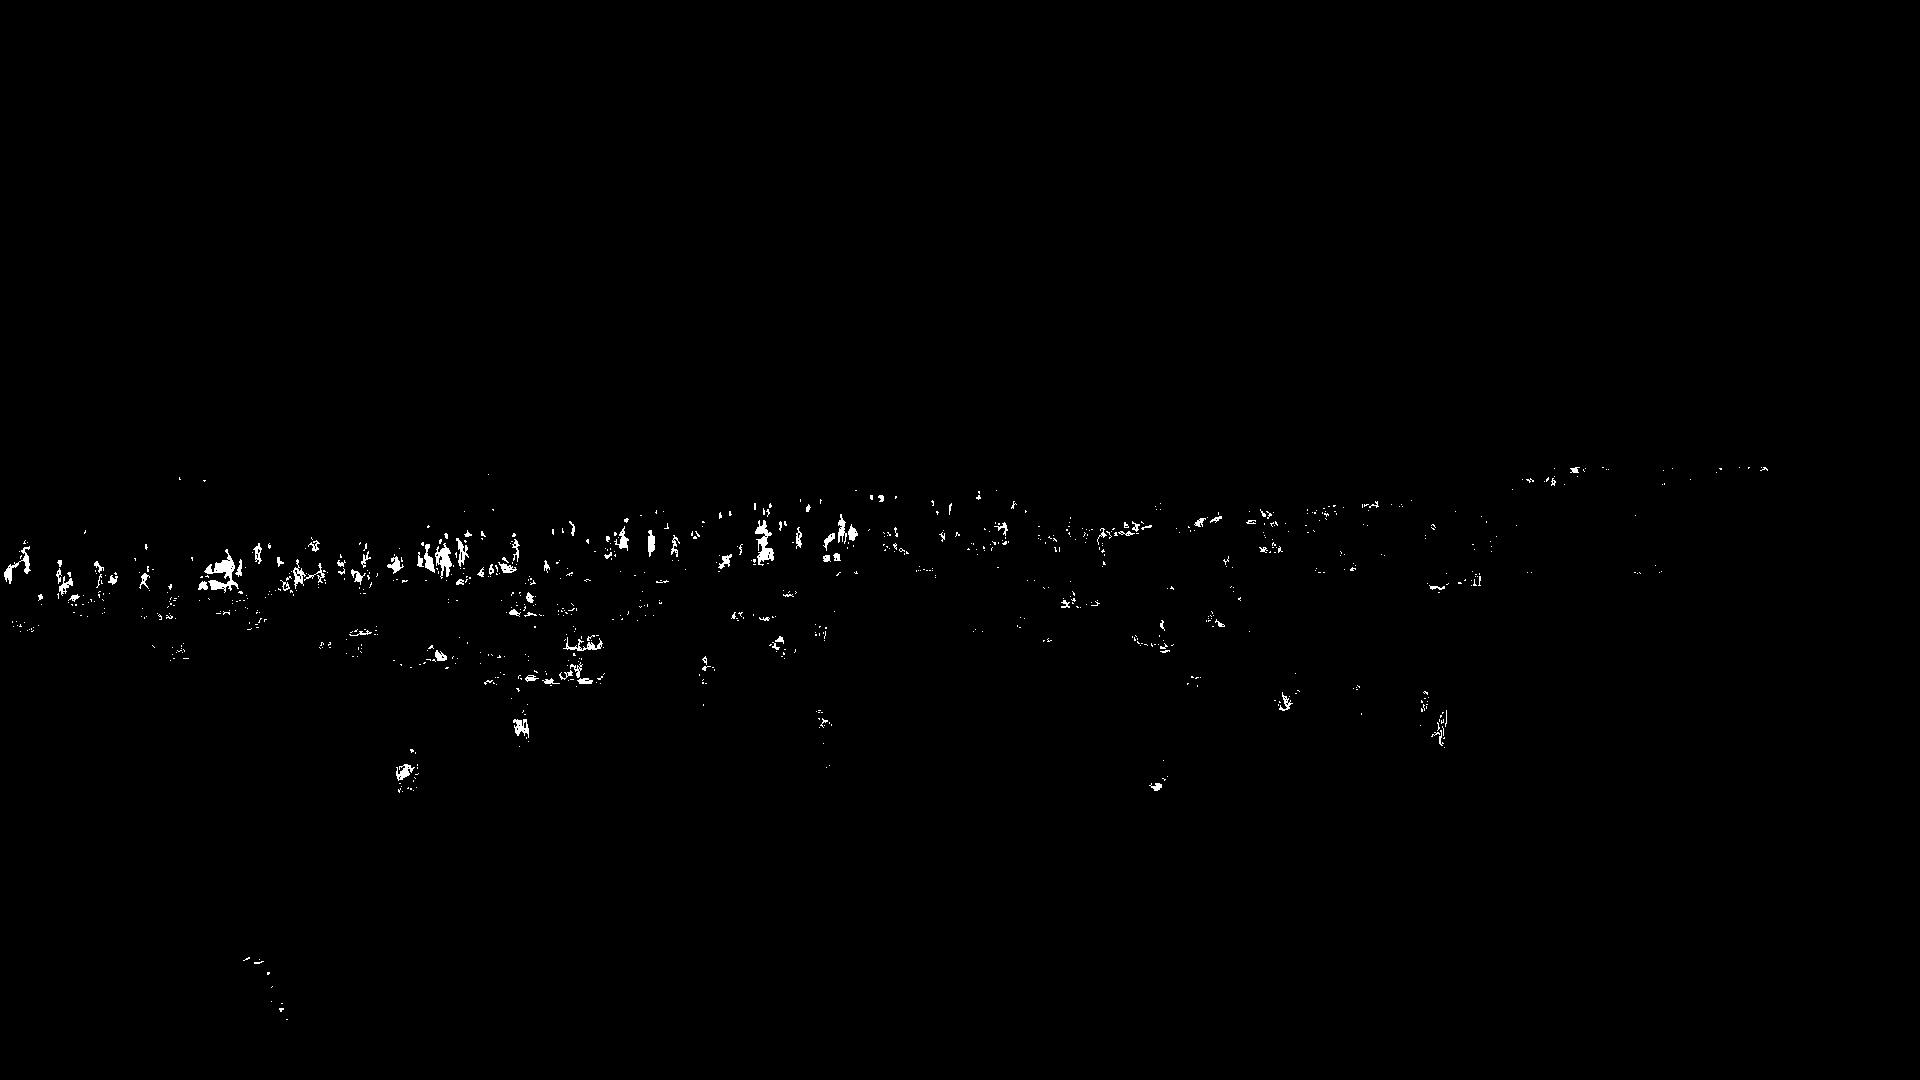
\includegraphics[width=\textwidth]{img/bin_ex.jpg}
    \caption{Output of background substraction using cv2.threshold(image, 100, 255, cv2.THRESH\_BINARY)}
    \label{fig:y equals x}
  \end{subfigure}
  ~
  \begin{subfigure}[t]{0.5\textwidth}
    \centering
    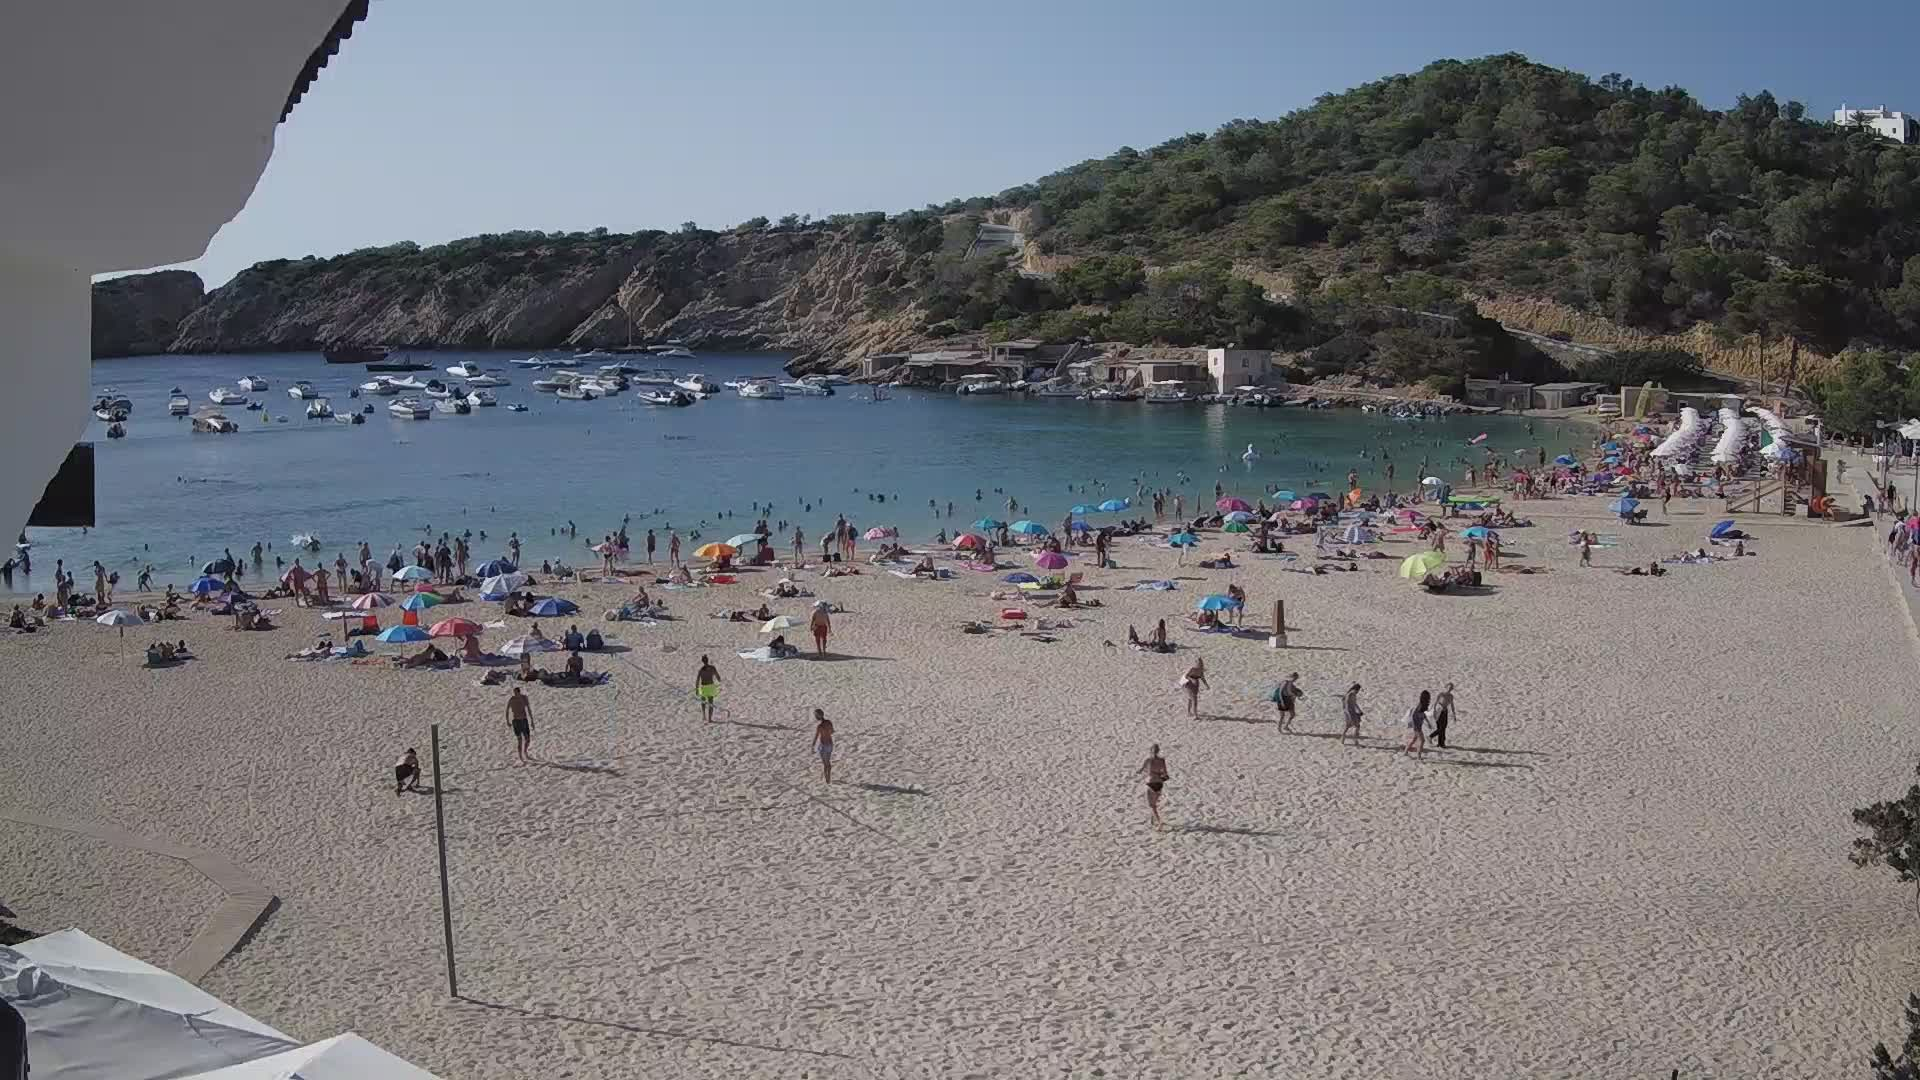
\includegraphics[width=\textwidth]{img/or_ex.jpg}
    \caption{Original 1660320000.jpg}
    \label{fig:y equals x}
  \end{subfigure}

  \caption{Reference images}
  \label{fig: img_reference}
\end{figure}
\FloatBarrier
In the following sections will be explained how the preprocessing of this technique was prepared and for what they are used for. They are ordered by

\subsubsection*{CLAHE}

In the case of our problem, first we have imported all the images in black and white integer values using \codeword{cv2.imread(img,0)}. Then for a better extraction, it has been applyed an \textbf{algorithm of CLAHE} seen previously on the course to try to uniformize the ilumination of the images. With a more uniform images, we will be able to distinguish more precisely our foreground and artifact like shadows casted by objects on the images may have less impact on the \textbf{binarization process}.

\begin{figure}[h]
  \centering % <-- added
  \begin{subfigure}{0.25\textwidth}
    
\includegraphics[width=\linewidth]{img/equ/1660284000.jpg}
    \caption{1660284000.jpg with CLAHE applyed}
    \label{fig:1}
  \end{subfigure}\hfil % <-- added
  \begin{subfigure}{0.25\textwidth}
    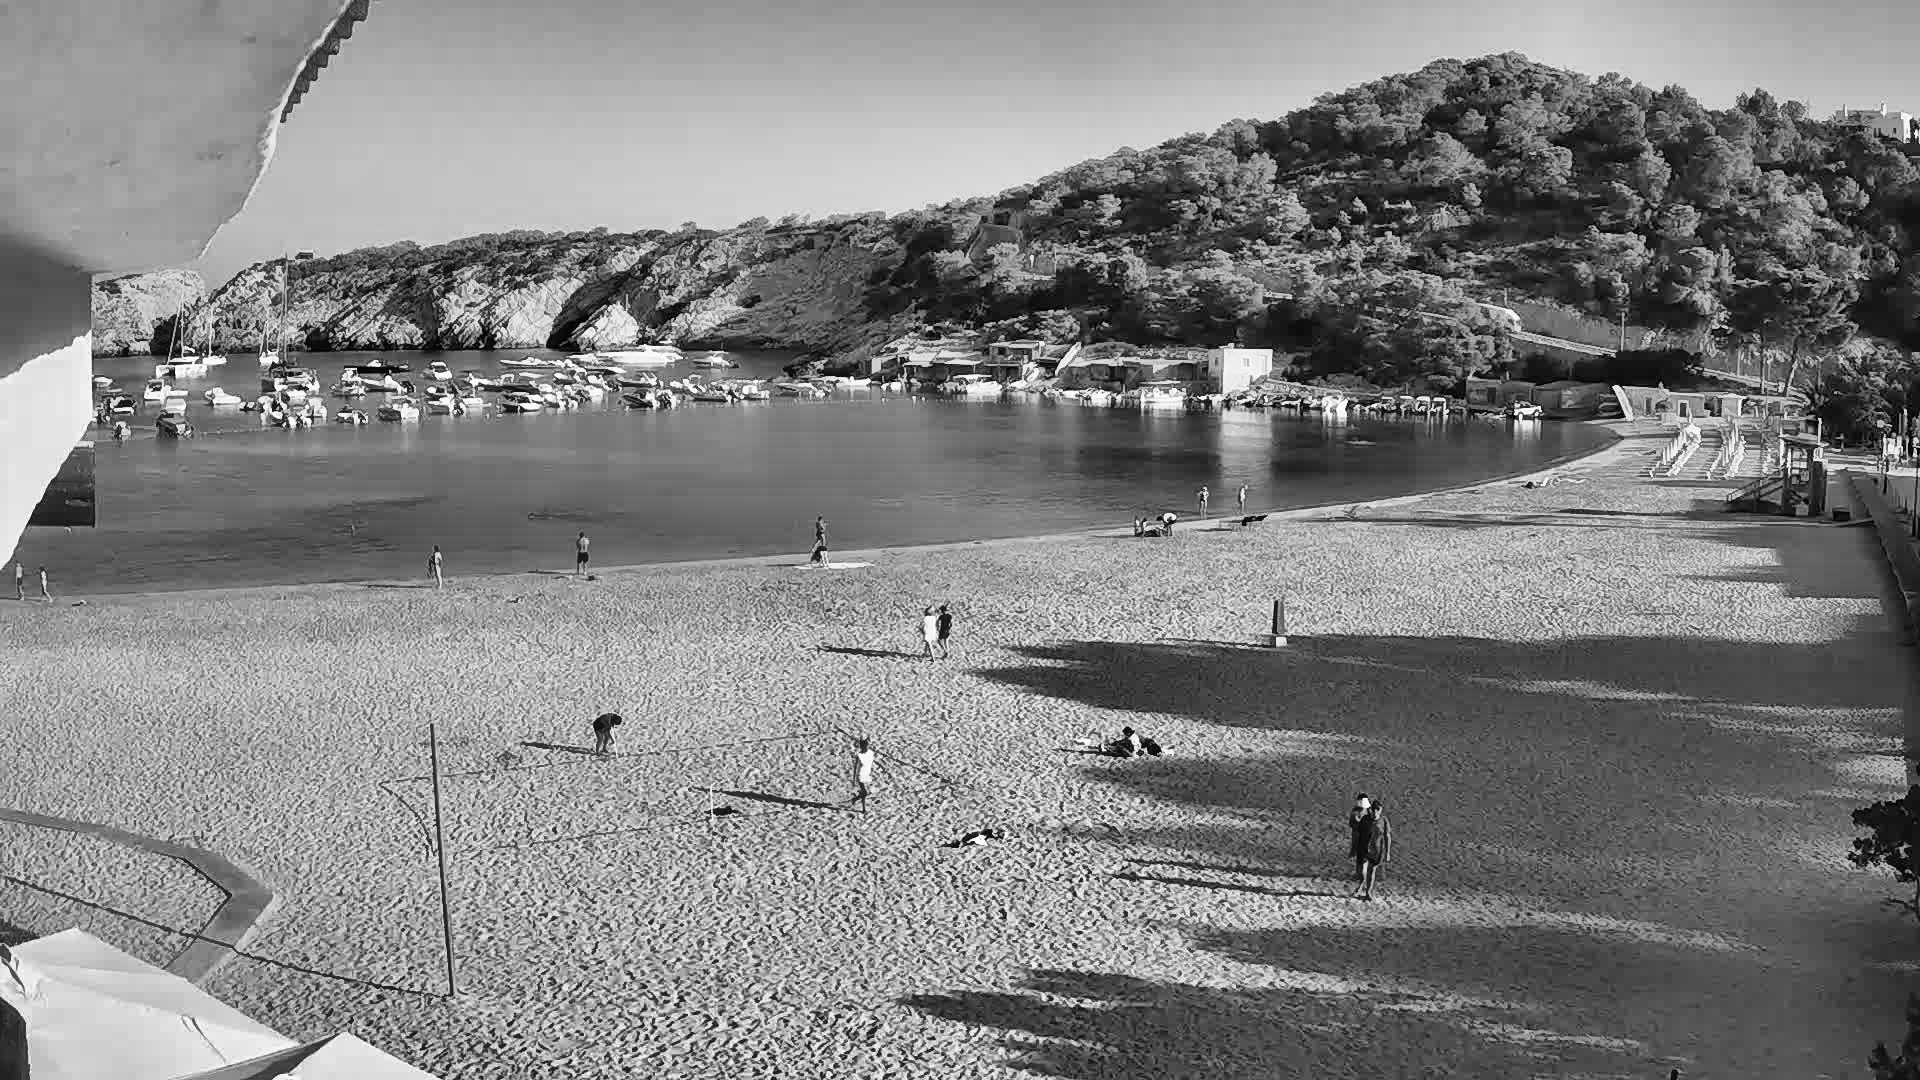
\includegraphics[width=\linewidth]{img/equ/1660287600.jpg}
    \caption{1660287600.jpg with CLAHE applyed}
    \label{fig:2}
  \end{subfigure}\hfil % <-- added
  \begin{subfigure}{0.25\textwidth}
    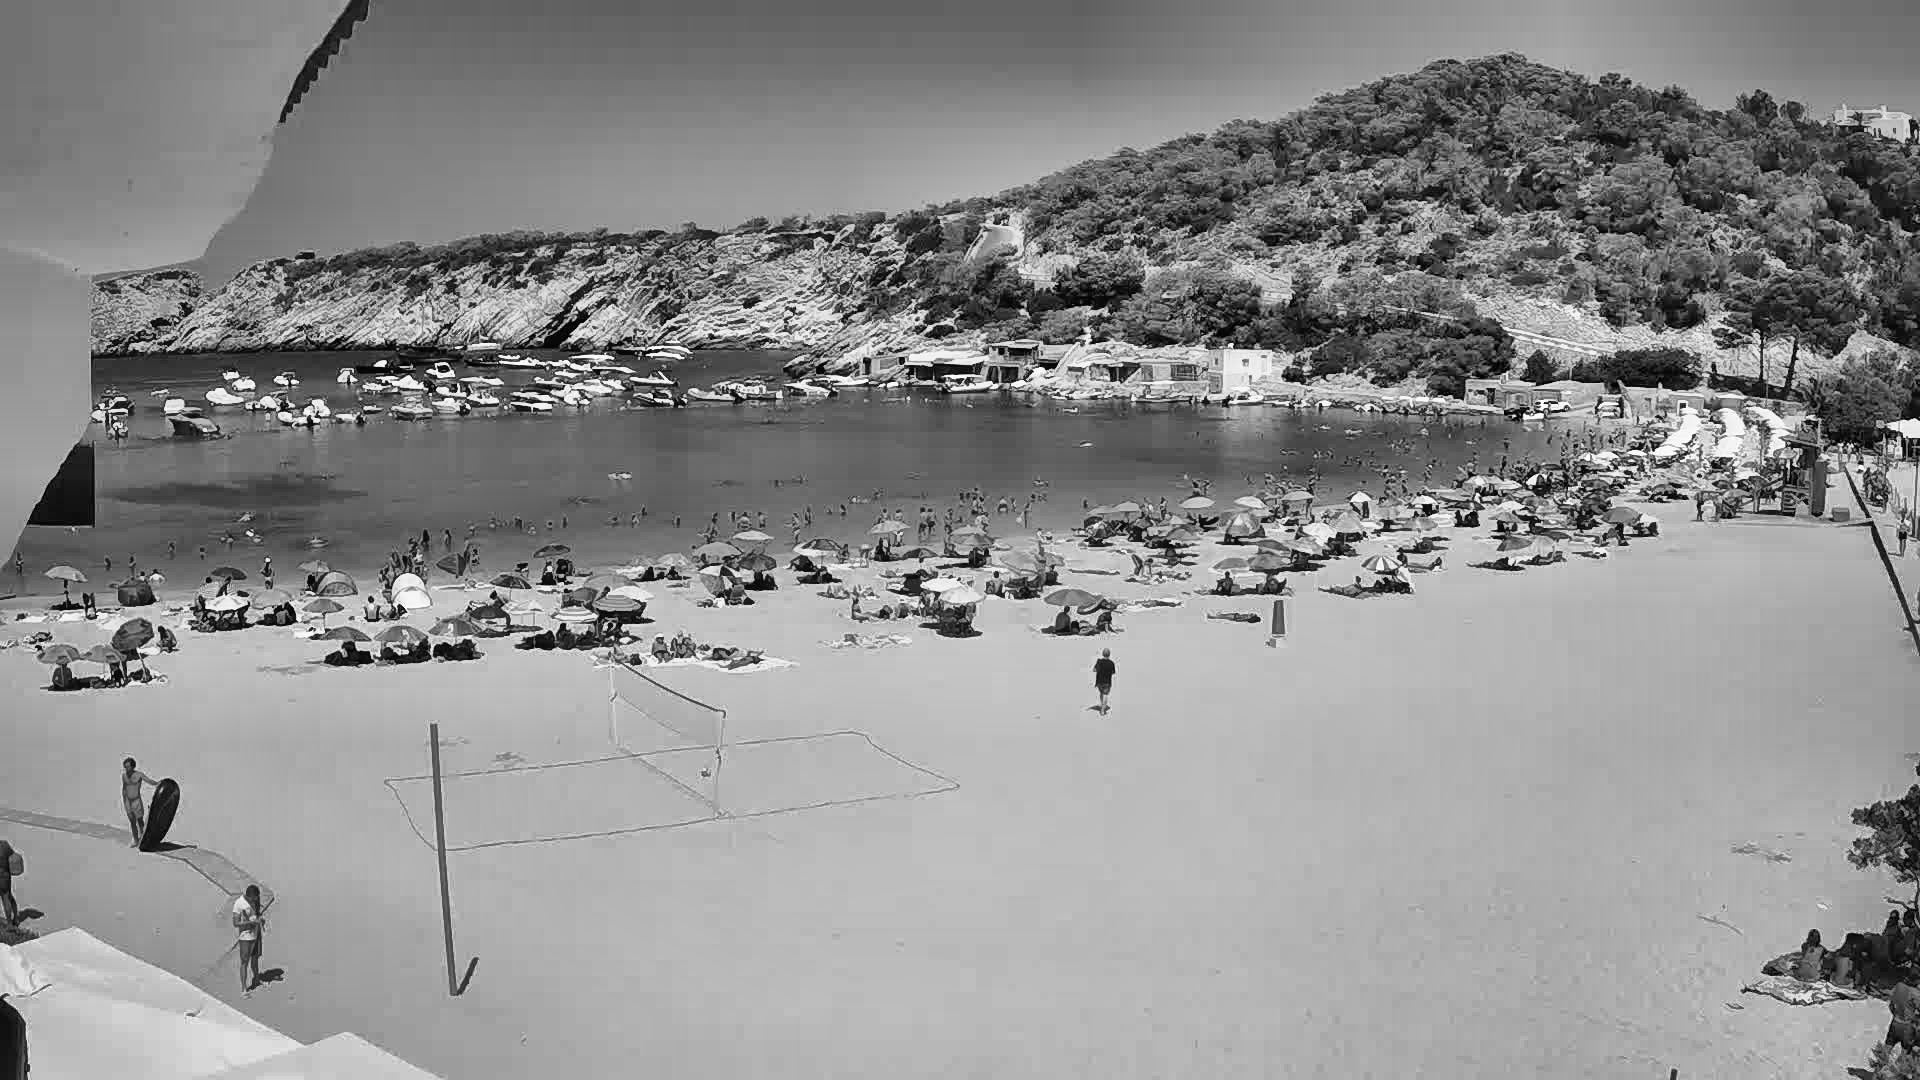
\includegraphics[width=\linewidth]{img/equ/1660302000.jpg}
    \caption{1660302000.jpg with CLAHE applyed}
    \label{fig:3}
  \end{subfigure}

  \medskip
  \begin{subfigure}{0.25\textwidth}
    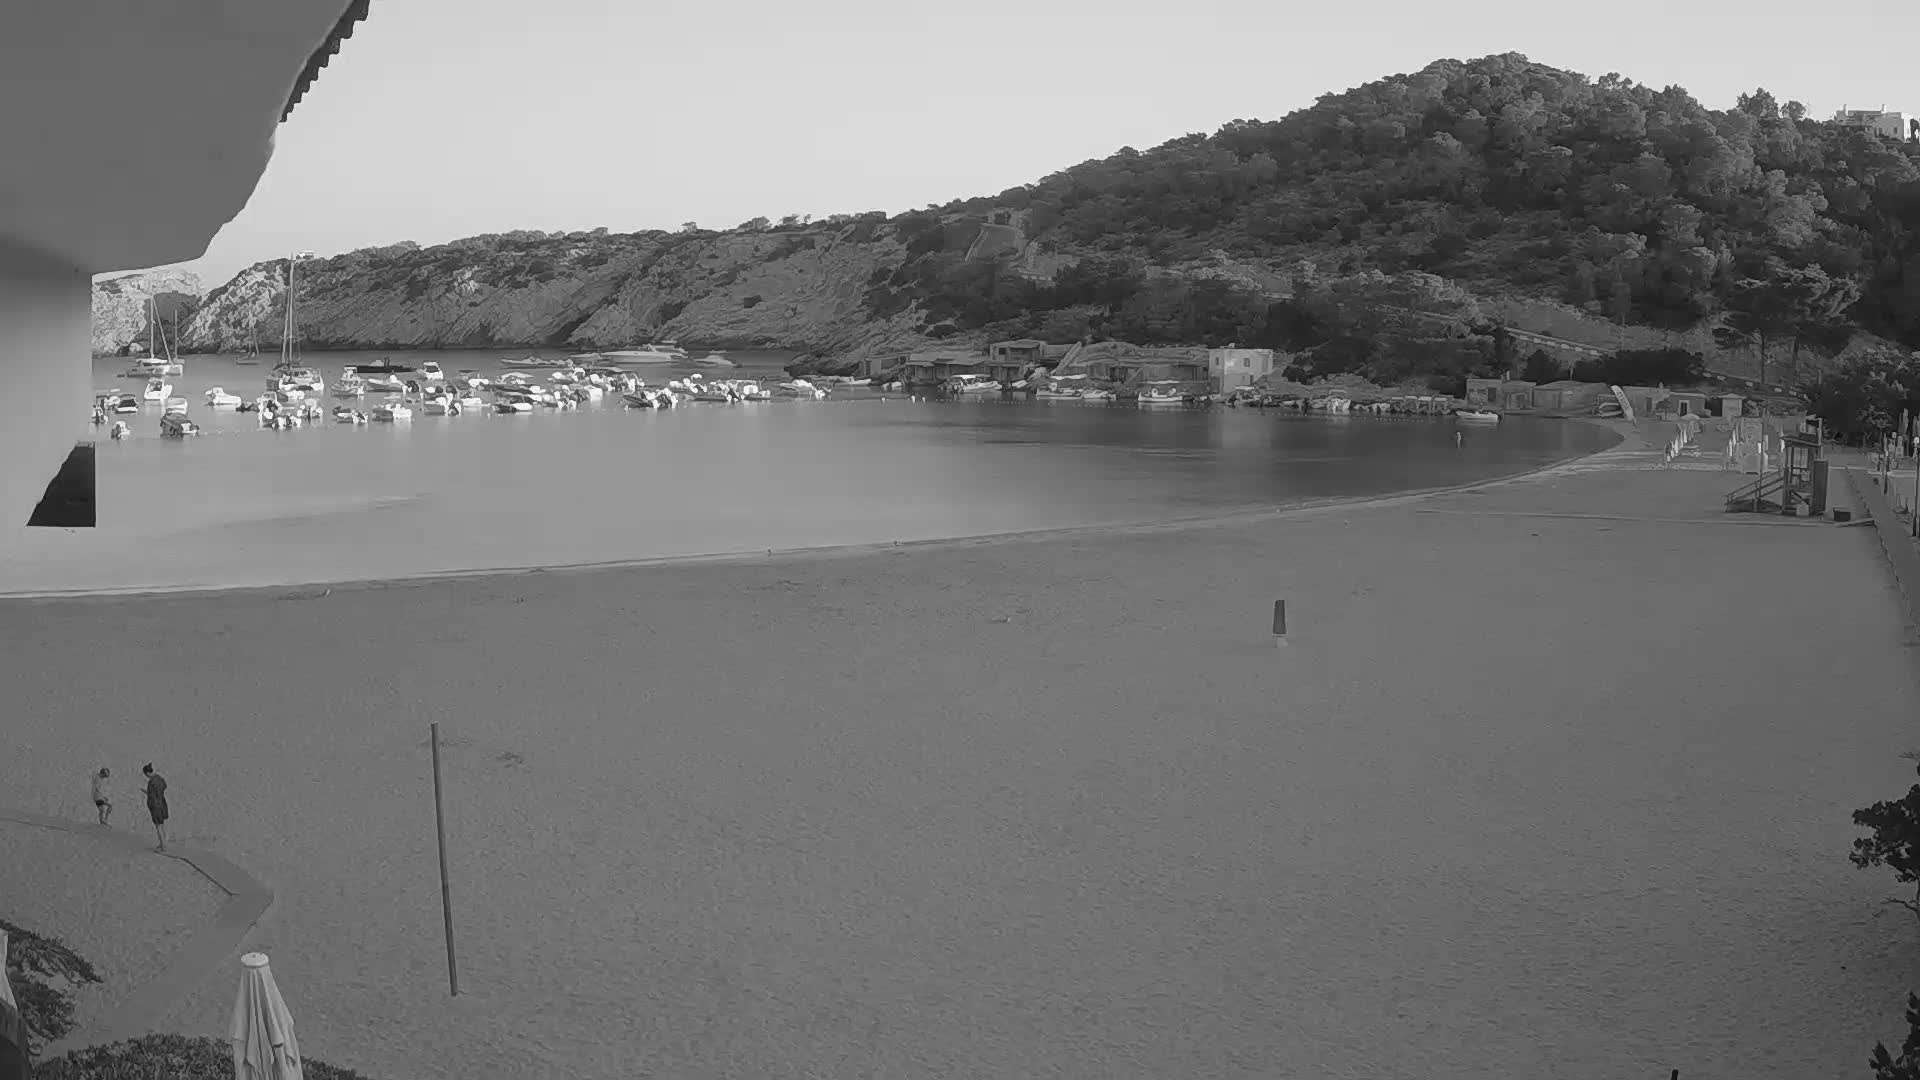
\includegraphics[width=\linewidth]{../gen/gray/1660284000.jpg}
    \caption{1660284000.jpg gray}
    \label{fig:4}
  \end{subfigure}\hfil % <-- added
  ~
  \begin{subfigure}{0.25\textwidth}
    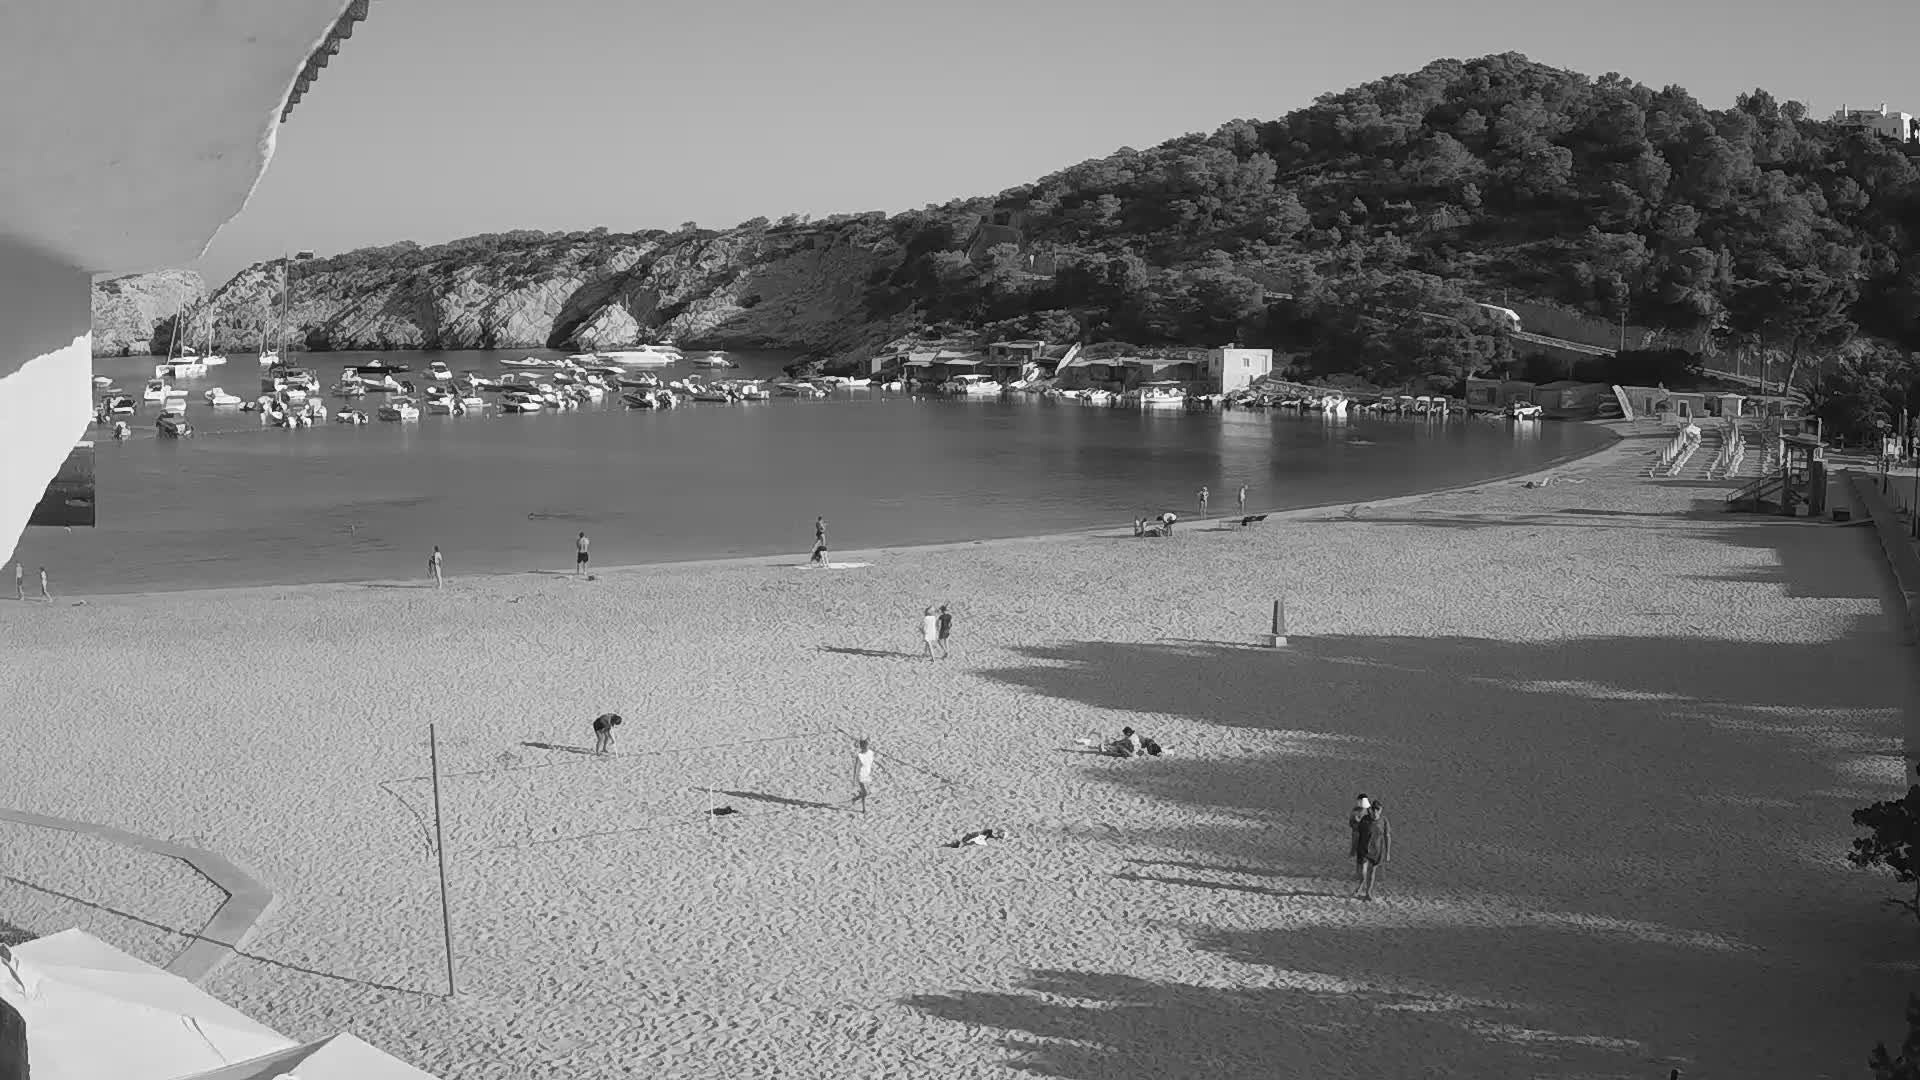
\includegraphics[width=\linewidth]{../gen/gray/1660287600.jpg}
    \caption{1660287600.jpg gray}
    \label{fig:4}
  \end{subfigure}\hfil % <-- added
  ~
  \begin{subfigure}{0.25\textwidth}
    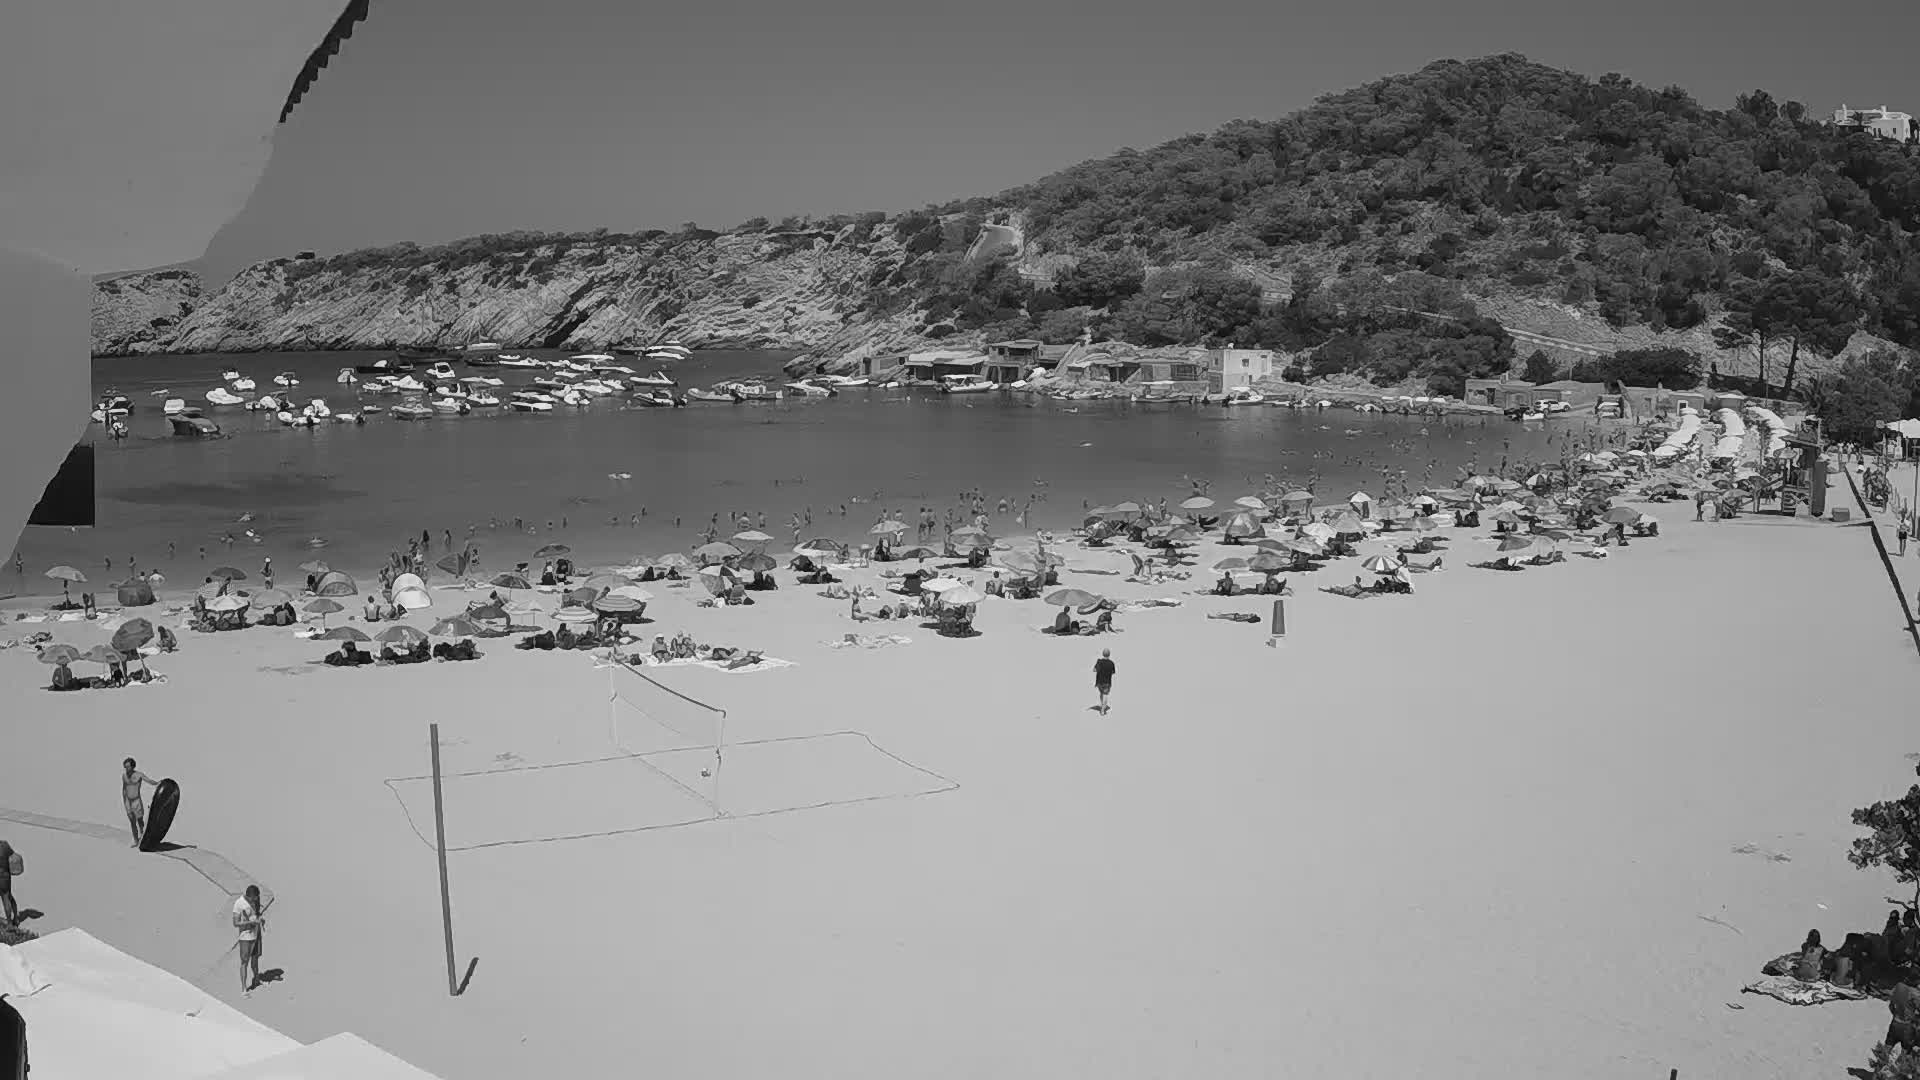
\includegraphics[width=\linewidth]{../gen/gray/1660302000.jpg}
    \caption{1660302000.jpg gray}
    \label{fig:4}
  \end{subfigure}\hfil % <-- added
  \caption{Images from Gelabert folder where the first row presents a more uniform ilumination across frames ompared with the second row images.}
\end{figure}

\FloatBarrier
\subsubsection*{Background Image}

For the selection of our background image, in a starting point the \textbf{average image} was computed as the main way for accomplish foreground extraction, but the resulting image generally was really noisy and with ghosting effect very present on it, which decreased the performance of the algorithm as it can bee seen on the Figure \ref{fig:avg}. Even with a gaussian blur applyed to try to counter the ghosty figures, they are still really present on the image. The image averaging is a good idea generally for noise reduction and in this case to try to obtain a neutral image were the background is predominant, but there is not enought images to obtain a more sharp image to really have a good background. Therefore, we \textbf{end up} using the image 1660284000.jpg with a gaussian blur applyed as our background, this way we obtain better results on the \textbf{binarization process}.

%\begin{figure}[h]
%    \centering
%    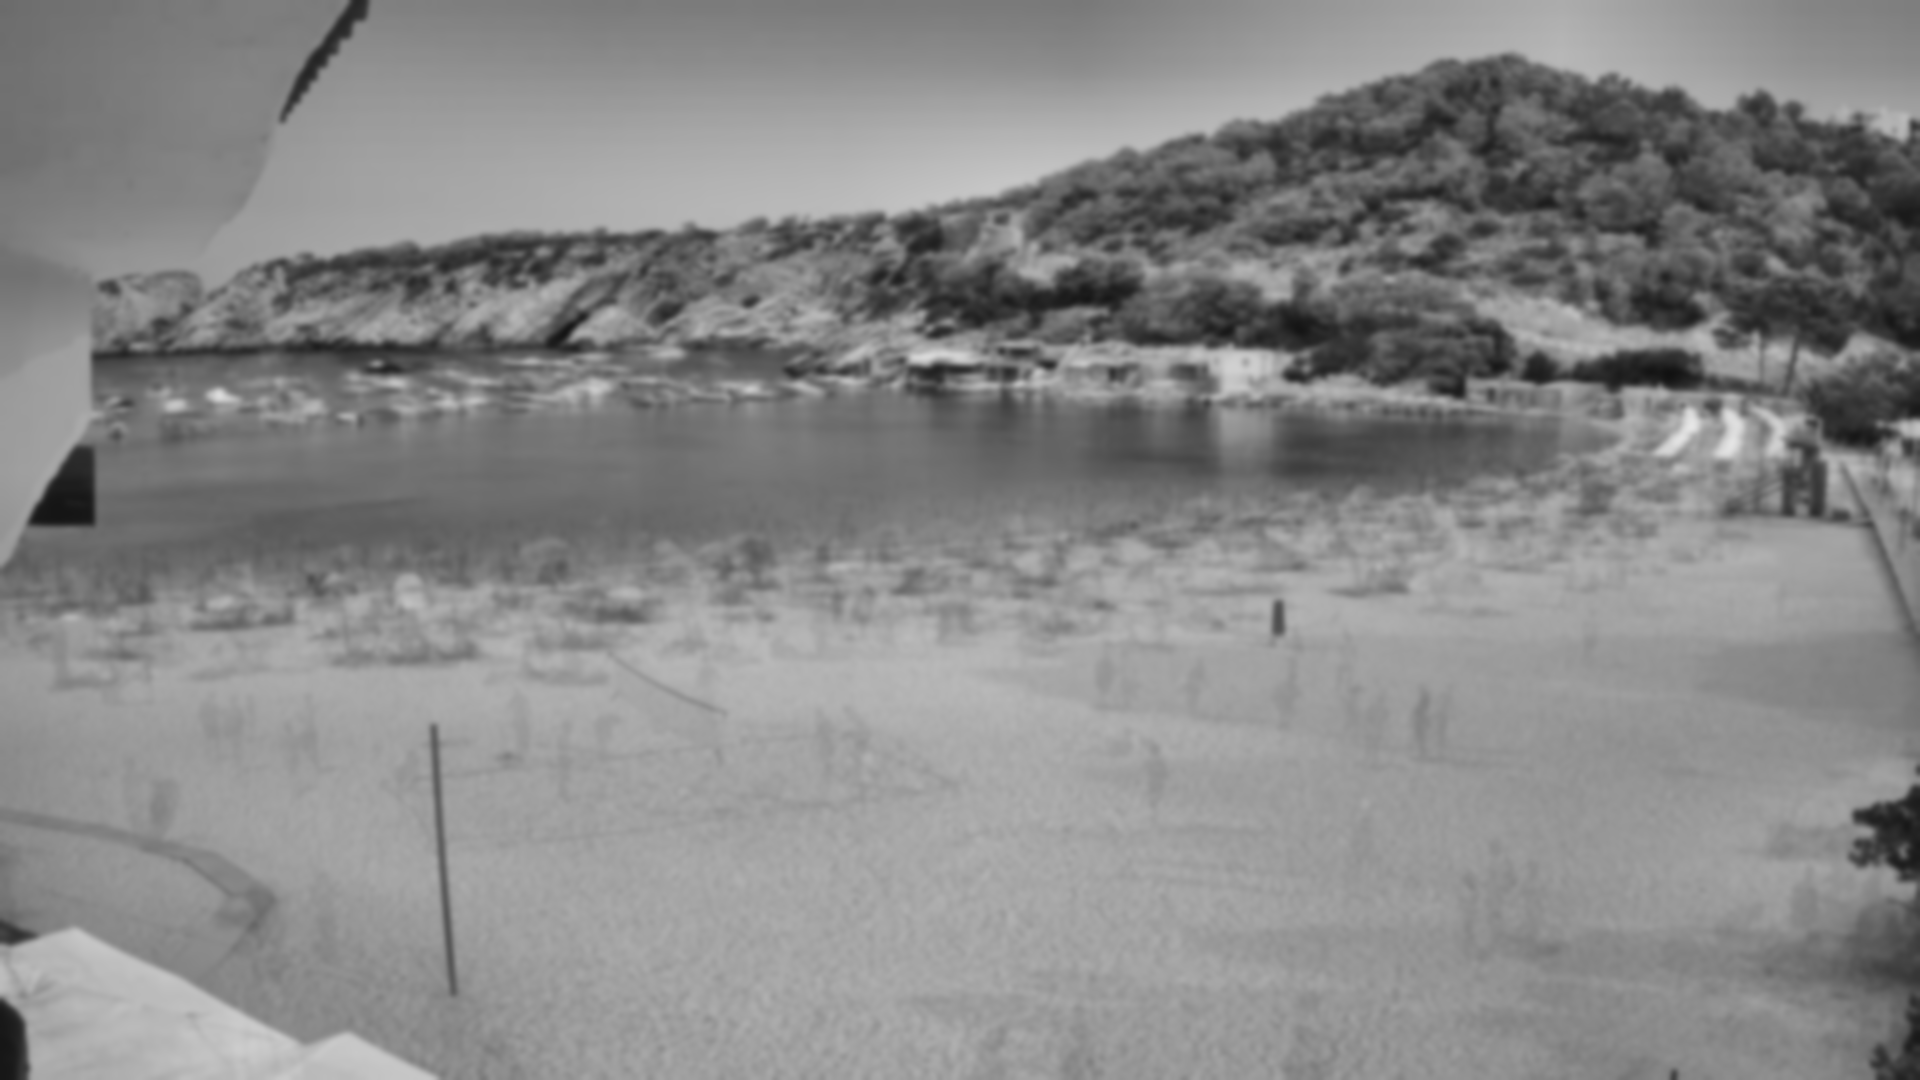
\includegraphics[width=0.9\textwidth]{img/avg.png}
%    \caption{Average image with a gaussian blur applyed with a kernel of (11,11)}
%    \label{fig:avg}
%\end{figure}



\subsubsection*{Gaussian Blur}
With an image already selected for the image background, it is applyed a gaussian filtering with a kernel of size (7,7), this way  we can obtain a more standard image, and get a more smuthered image that will allow the algorithm to contrast slightly better our foreground.\newline

%\begin{figure}[h]
%    \centering
%    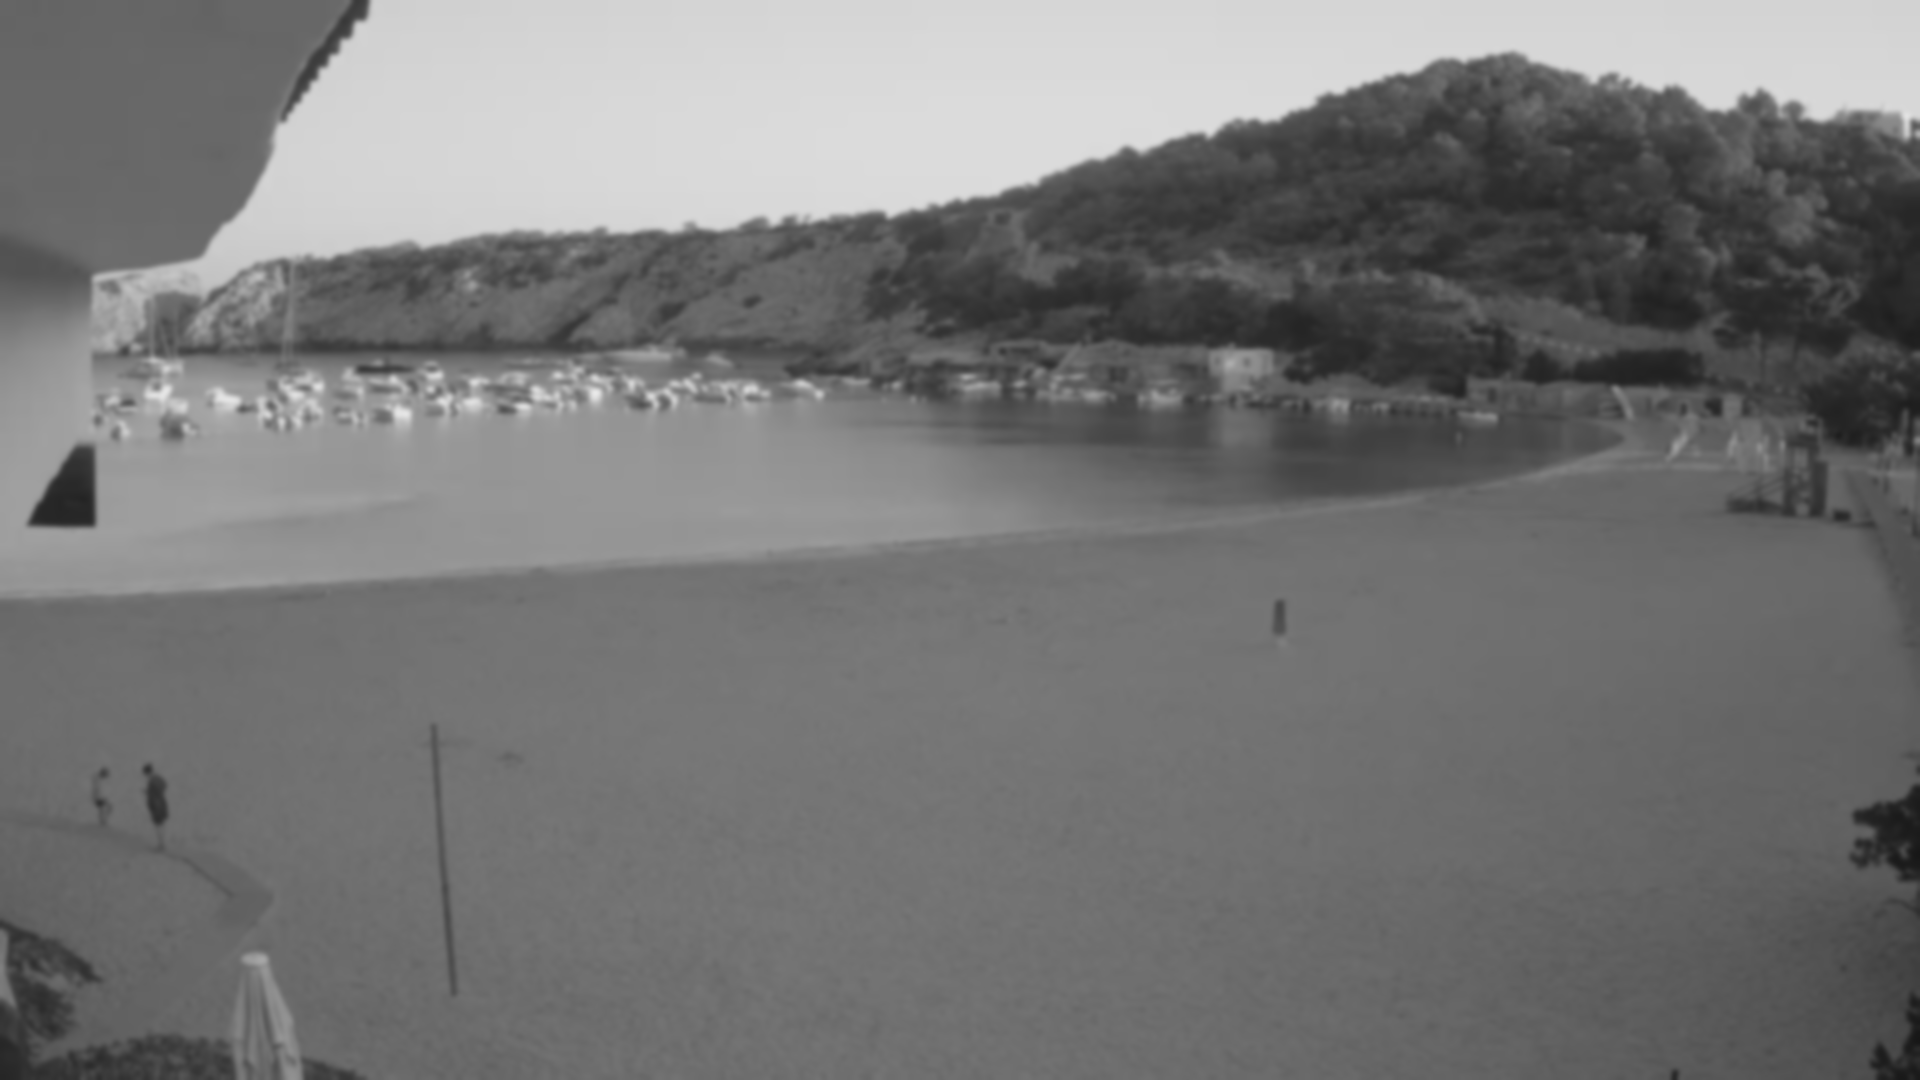
\includegraphics[width=0.9\textwidth]{img/back_blur.png}
%    \caption{Gaussian Blur Applyed with a kernel of size (7,7)}
%    \label{fig:gaussian}
%\end{figure}



The ending size used for gaussian blur was obtained by trial and error experimentation, and could be changed to get different ending behaveours.


\subsubsection*{Substraction}

Once we have selected our background and applyed the preprocessing, we should substract it to every image, this way, the result we end up with is the foreground (in this case the persons and some residuals) highlighted as we can see in the figure \ref{fig:sub}.

%\begin{figure}[h]
%    \centering
%    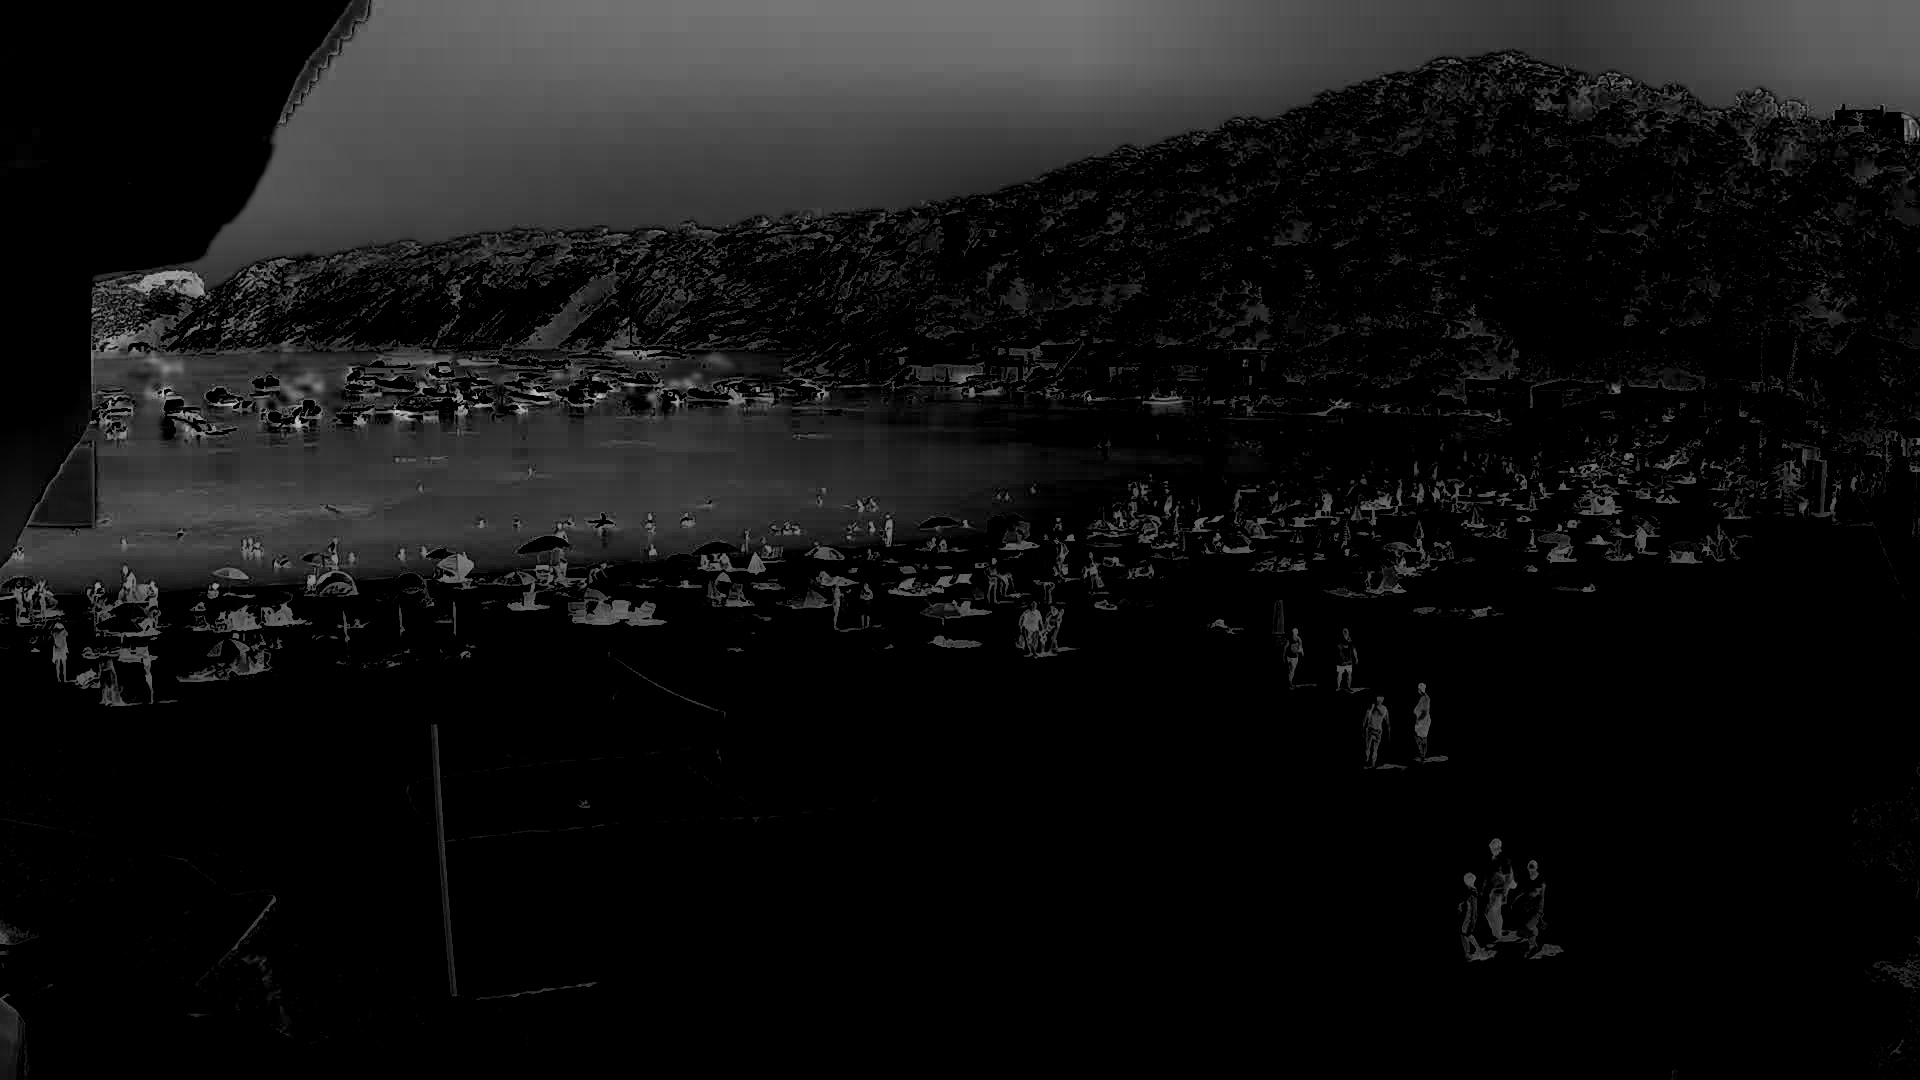
\includegraphics[width=\textwidth, height=\textheight, keepaspectratio]{img/sub.jpg}
%    \caption{Image obtained by applying cv2.subtract(background, image)}
%    \label{fig:sub}
%\end{figure}


\subsection{Binarization}
Once the substraction has been aplyed to all images, the resulting foreground will contain hopefully our persons. All those whity areas should be further treated using a binarization progress, allowing a solid division between  the background and our foreground. This is acomplish by the process of binaryzation. Depending of the process selected, the resulting image will transform into a binary black and white image from a gray scale one. In this assignment there has been some experimentation using OTSU and the binary threasholding function avaliable on cv2 library, but for the sake of the performance, the last one has been ultimately selected.\newline

The problem with using OTSU is that for each images it obtains a threshold selection automatically, and this should not be a problem, and sometimes could perform better than a fixed one. But for the samples tested there are a lot of artifacts related to the shadow casting of the image, as it can be seen in the figure \ref{fig:otsu_bin}. The problems are seen on the bottom of the image, where there are an amount of shadows casted by the sand crests which can be a bit annoying for the next steps.\newline


%\begin{figure}[h]
%    \centering
%    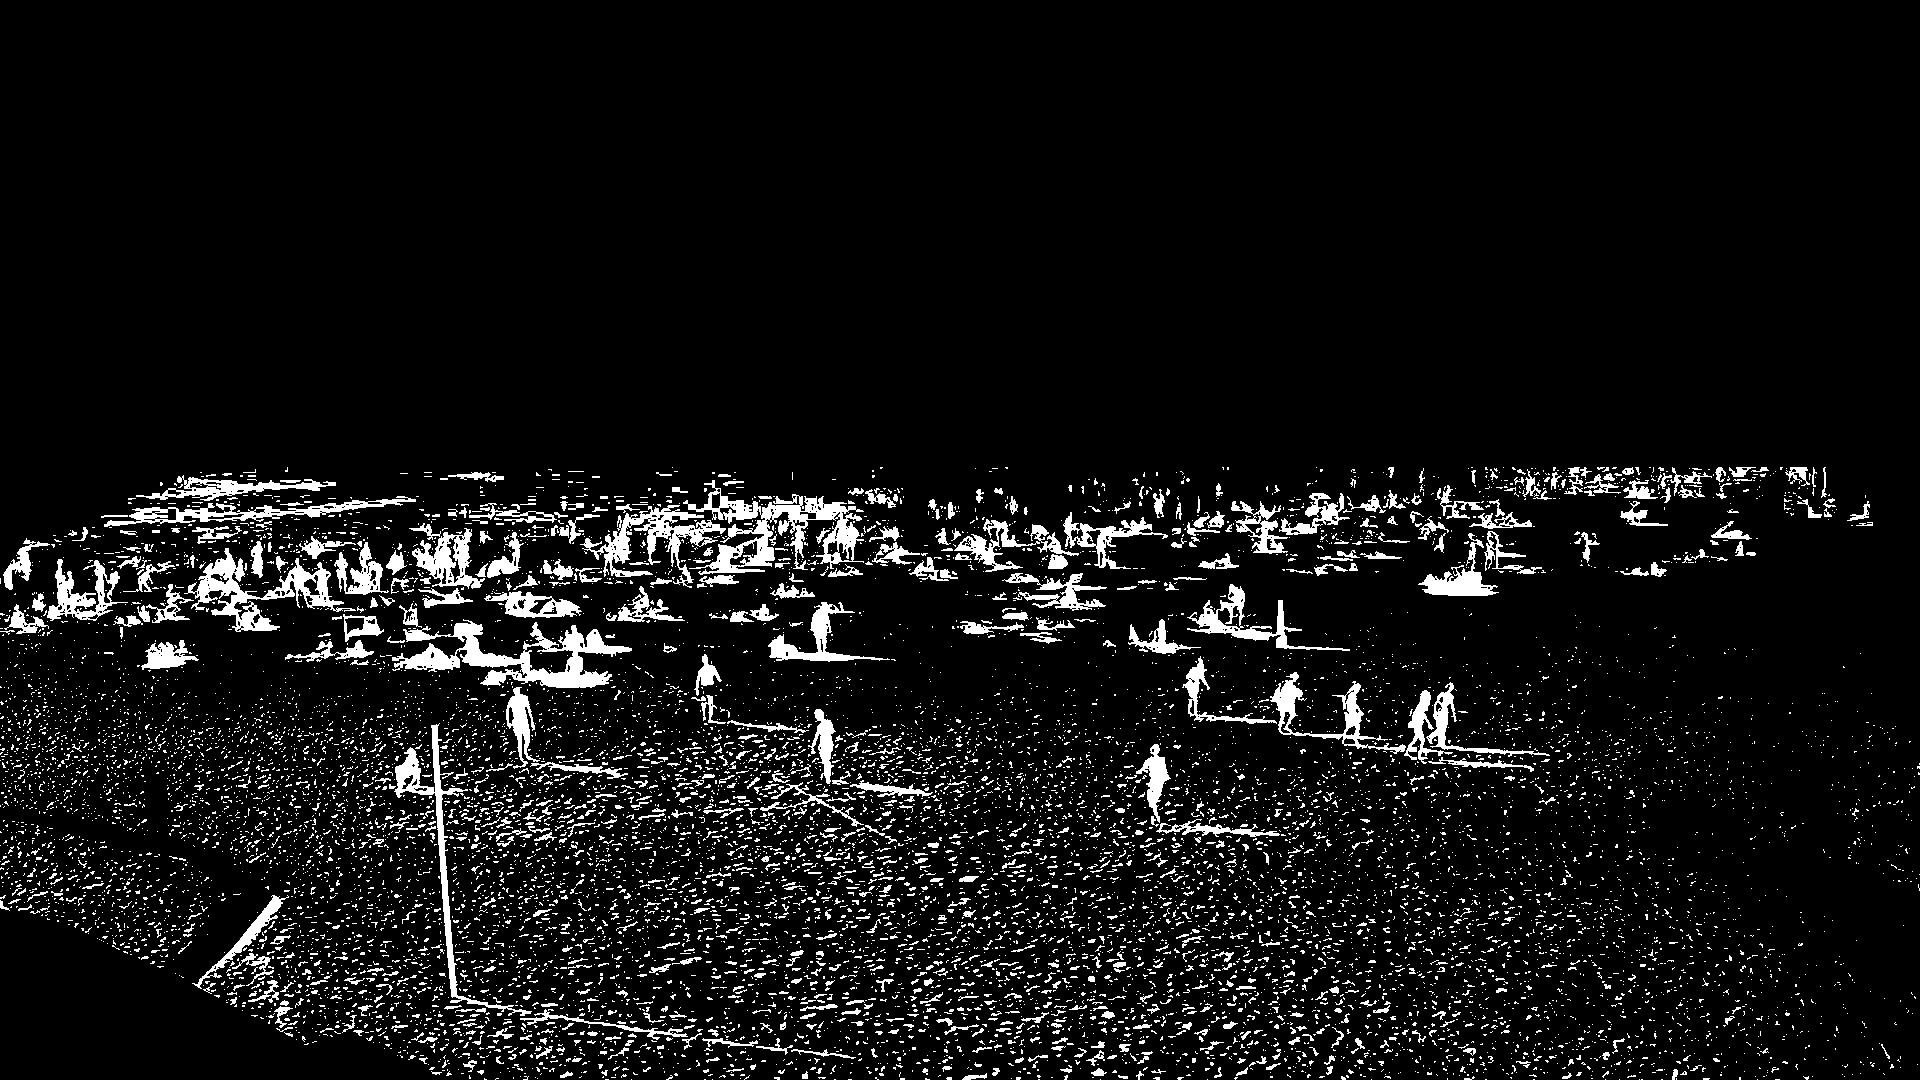
\includegraphics[width=\textwidth]{img/OTSU_sub_arena.jpg}
%    \caption{Binarized image using OTSU and the empty beach image}
%    \label{fig:otsu_bin}
%\end{figure}

%\FloatBarrier


By using a set thresholding we are loosing some flexibility and a fixed values could not be the wiser idea, but in this case using a tigth threshold may be the best decision as may reduce the number of false detections considerably. In this case the values selected are setted in the instruction \codeword{cv2.threshold(substracted, 100, 255, cv2.THRESH_BINARY)}. The resulting image can be shown in figure \ref{fig:binth}.


%\begin{figure} [hp]
%    \centering
%    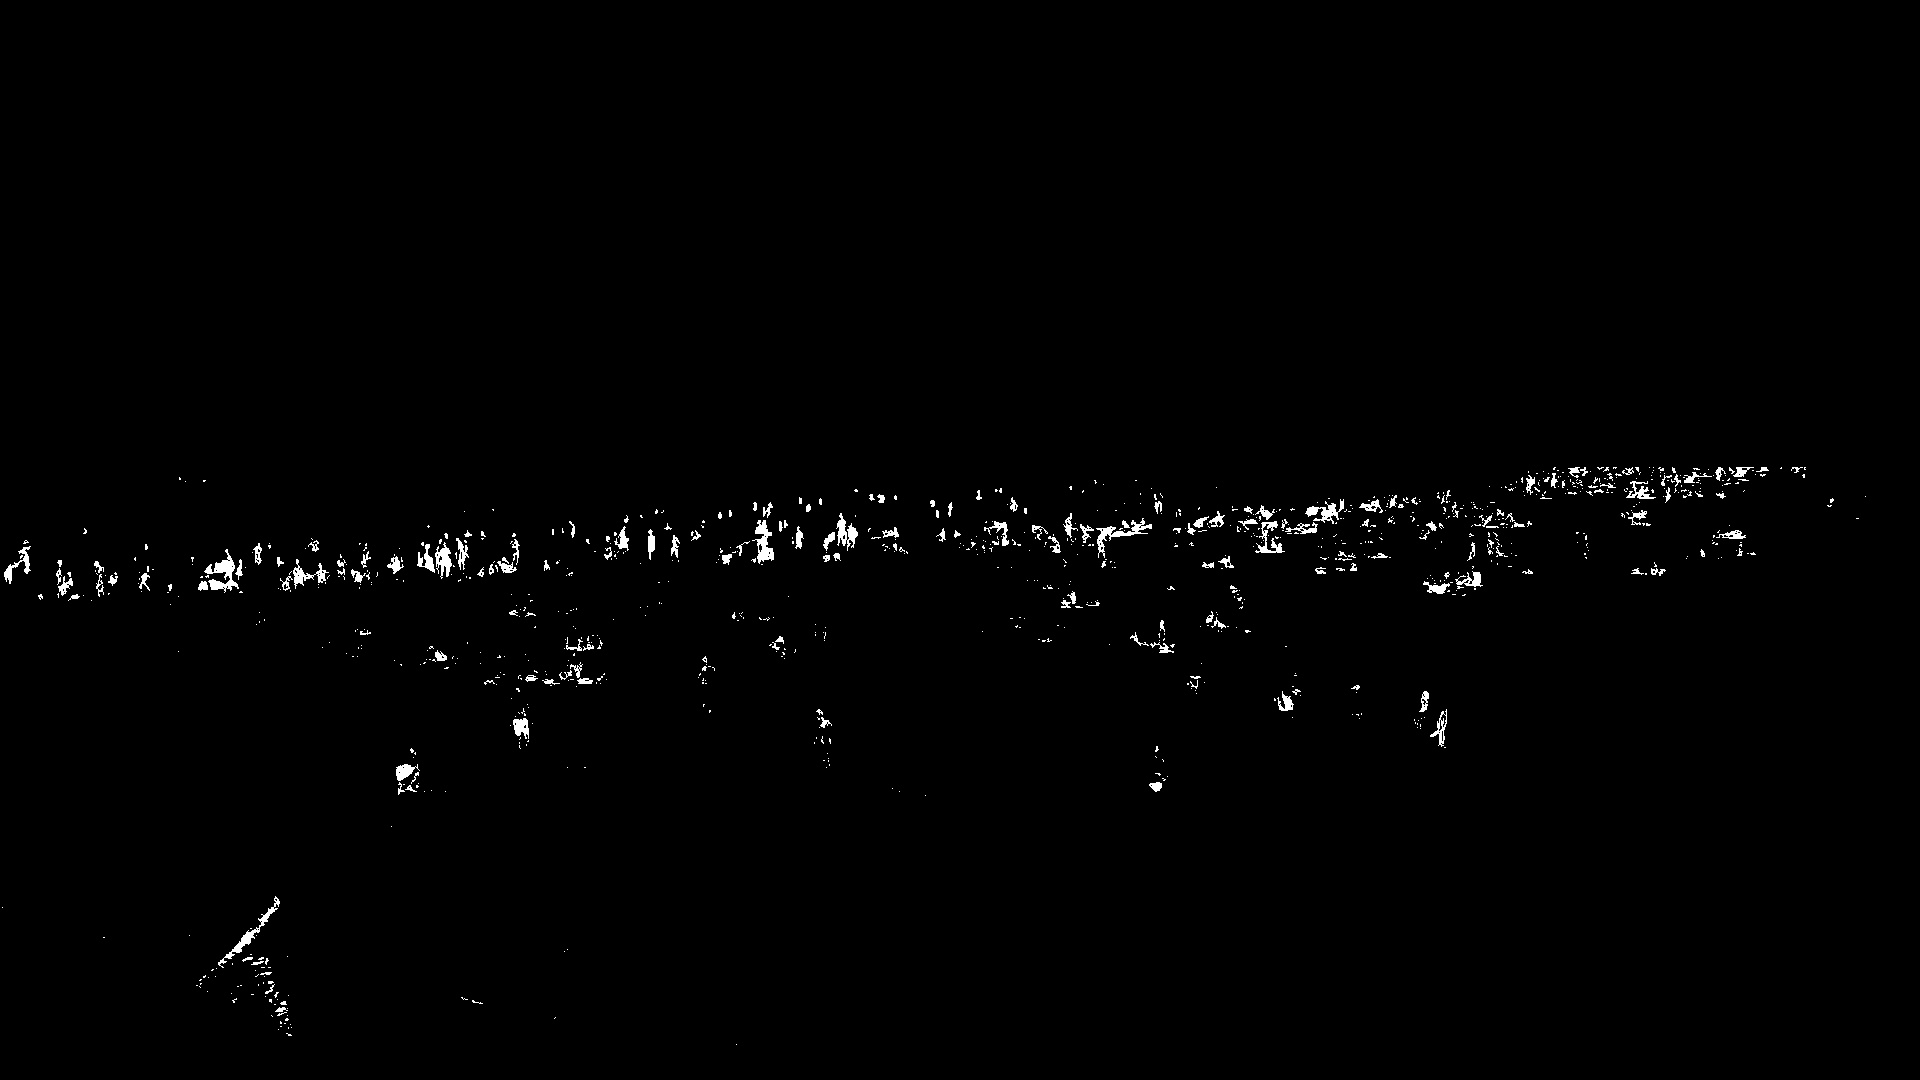
\includegraphics[width=\textwidth]{img/bin_th.jpg}
%    \caption{Binarized image using a fix thresholding method}
%    \label{fig:binth}
%\end{figure}

\subsubsection*{Masking}
For a better filtrage of our data, we will be using a binary mask to get rid of centain areas of the image where we can get non-persons in the foreground (i.e the quay part) and those areas where there is to much information to get clear data about it. We can see the last case in the umbrella section of the beach and the pavement area, where there are too many persons overlaping each others. The mask applyed can be seen in the figure \ref{fig:mask_ex}.



\subsection{Dilation}
Now, with the image binarized we will a apply a dilation to the image. The dilation will expand the white color on a binarized image, obtaining as results the highlighted areas in form of white chunks as it can be seen on figure \ref{fig:dilation_ex}. With these chunks the countourn detection will obtain better results because they are more clear shapes. This could merge figures into one, so the parameters of the kernel size may be tinkered with to obtain the best performance possible.



\subsection{Find contours}
Once a binarized image is obtained, there should be a process of contour detection. Here we use the dilated images over the function that openCV provides \codeword{cv2.findContours()}. From this functions, we can extract the bounding boxes that contain each of the object contours. In the figure \ref{fig:detections} appears the image with some bounding boxes applyed.

%\subsection{Matching Algorithm}


\section{Results and Analysis}

For convenience, we will quantify our detection accuracy using the following assumptions:

\begin{itemize}
  \item If detection contains more than one person it will count as only one detection.
  \item In the case we would have a massive region we will discharge that detection.
  \item For checking the dimensionality of the bounding box, we would assume that width or height higher than a third of the image will not be acceptable.
  \item Regions minuscule will also be discarded.
  \item Some labels of the ground truth could be double checked.
        %For checking if the region detected contain labels inside their boundaries, only one will be check. In the case we would have a really big box keeping a lot of detection we will not count that as correct, but in the cases where it may contain a region of 4 or 5 persons because they are really close to each other, we would be more flexibles.
\end{itemize}
%For checking the dimensionality of the bounding box, we would assume that width or height higher than a third of the image will not be acceptable, and the same for the ones no more than two pixels size. 

The reason of the anterior list, are bounded to the complexity of the problem. We are not restrictive enought to loose a lot of information. Allowing more flexibility in order to have more valid detections let us obtain a better performance overall. Also, some cases are unlikely to happen really offen. In the tables \ref{table:metrics1} and \ref{table:metrics_2} is shown how the algorithm performs.

\subsection*{Results}

In table \ref{table:metrics1}, the column of \textit{gt} represent the number of labels on each image, \textit{detected} represent the number detections found in the image, and the column \textit{matched} represent the number of detections where at least contained one label of our ground truth. As we can see, the tables show a low scoring, having an unbalance in between the actual number of persons in each image and the detections, in figure \ref*{fig:detections} we can observe the output of the algorithm. But of course the general problem we will still have is the quantity of false positives we end up having in some images. Even the \textbf{mean squared error} with a value of \input{../MSE.txt} tells how this algorithm is having a huge error, we are predicting with a really soft constrains and allowing a lot of error on our detections. Although this is done entirely on purpose and in the practice this has turned our to be more beneficial for our images.\newline


\begin{table} [h]
  \centering
  \caption[Performance metrics Basic]{Performance metrics using the proposed algorithm}\label{table:metrics1}
  \csvautobooktabular{../metrics.csv}
\end{table}

\begin{table} [h]
  \centering
  \caption[Performance metrics overall]{Performance metrics overall using the proposed algorithm}\label{table:metrics_2}

  \csvreader[%
    tabular=|l|l|,
    respect underscore=true,
    no head,
    table head=\hline Metric & Scoring \\\hline,
    late after line=\\\hline
  ]%
  {../metrics_2.csv}{}%
  {\csvcoli & \csvcolii}%
\end{table}

\begin{figure}[h]
  \centering
  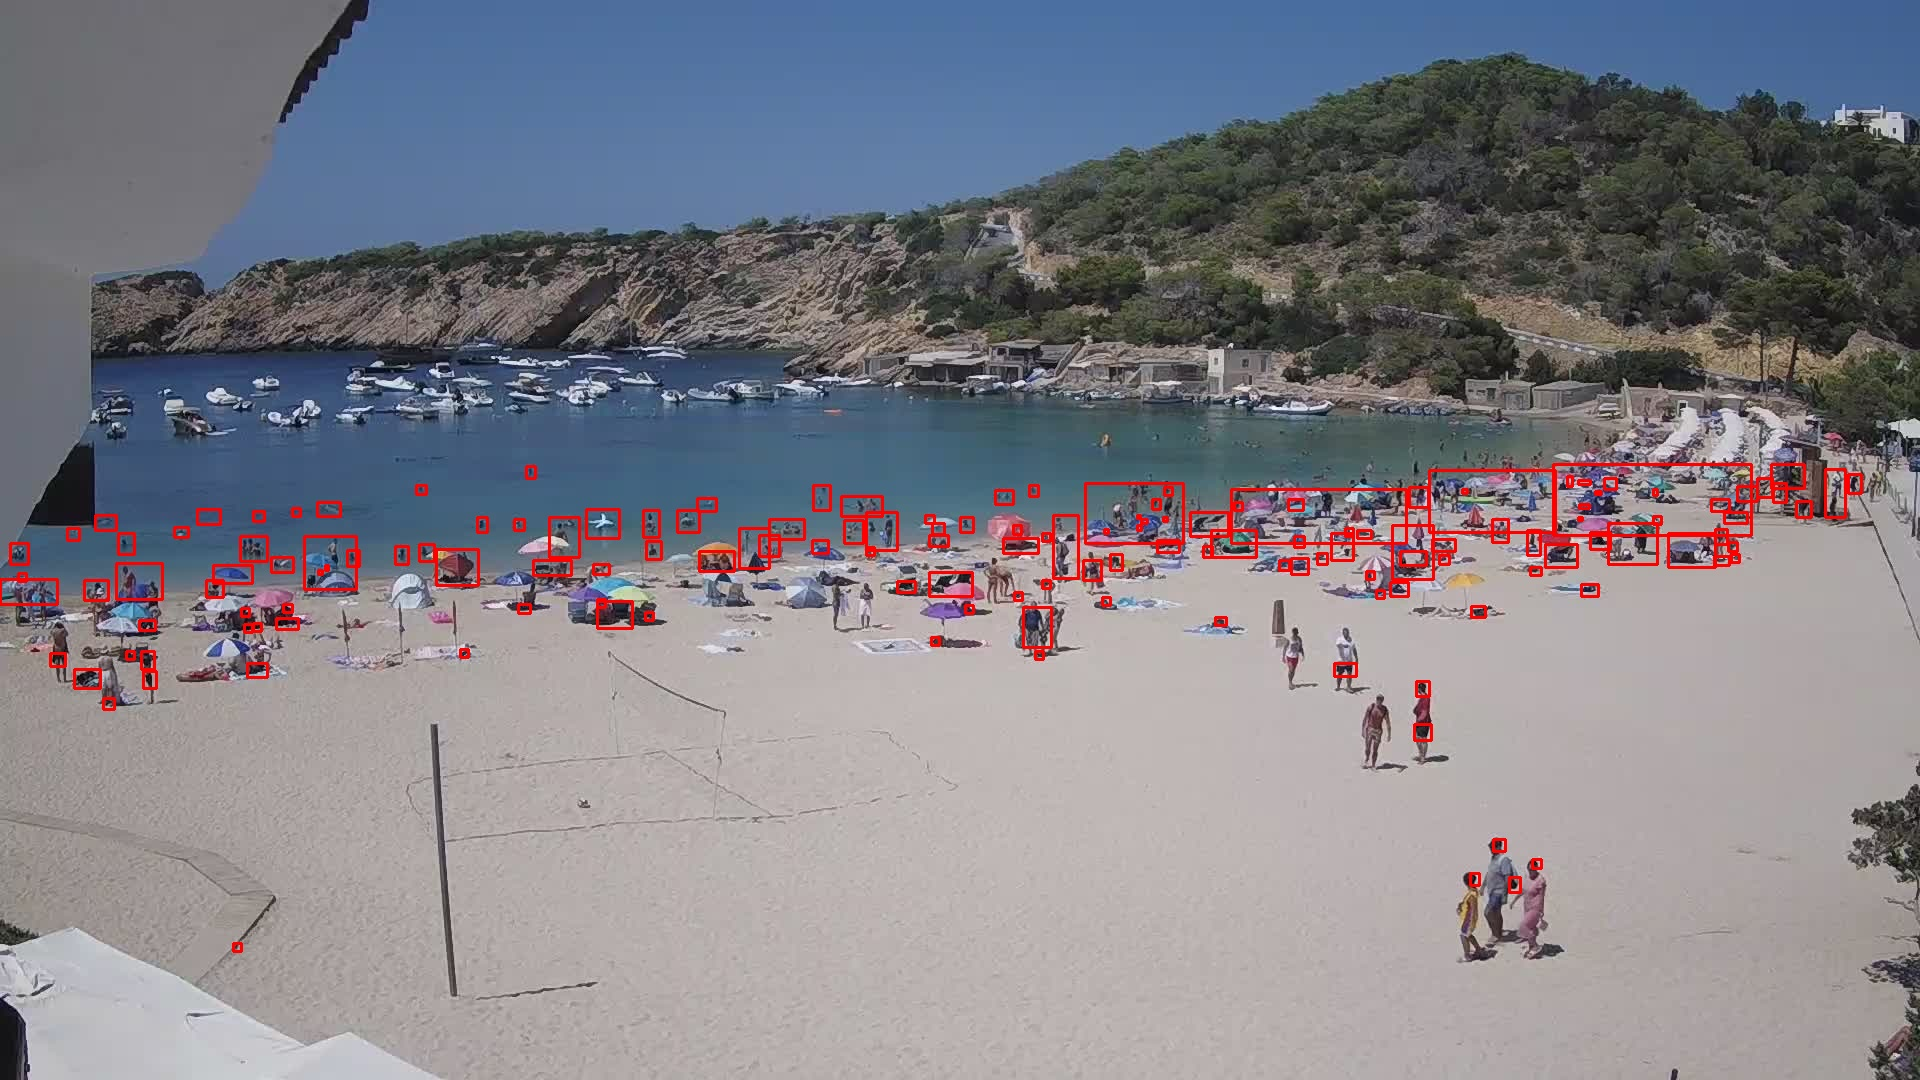
\includegraphics[width=\textwidth]{img/det_name.jpg}
  \caption{Output of foreground detector, as it can be seen there are some big detections due to contourn detecting multiple forms as one shape, and some }
  \label{fig:detections}
\end{figure}

\FloatBarrier


Should be considered that the type of images we got and the placement of the ground truth can make a huge difference on our outcome, so this algorithm has been tuned to try to be the more general possible \textbf{only} with the images provided in my corresponding directory.

\section{Is a different approach capable of improving our results?}

For some of the test that were executed for this assignment, generally the effort was not useful. Ending up in situations where a precise modification to the parameters gave as output excellent results only in a subset of the images. Usually the over-tunning of some function parameters made really inconsistent outputs that provoked a bad performance.\newline

In the following subsections it will be discussed some other paths to accomplish the task of the assignment, some of them had been implemented during the development stage if implemented or experimented with.

\subsection*{Color Spacing}

For example, one of the approaches taken for background removal, was the use of colored images in the color space of LAB  instead of gray scale. On the paper one may think that the use of color will improve our performance, because of the extra information we are just acquired from free. But in this case the process to obtain our foreground sections were in general less precise, giving as result a lot more objects as foreground, which is not ideal for our case, been a lot of those object just umbrellas and cast shadows.\newline

\subsection*{The problem with shadows}

In general, the sample images follow a consisting landscape withouth heavy cast shadows on the sand, but it is noticeable in some of them, and usually they will give you more than one headache.\newline

We could try to counter some cases using a sharpening processes or even more filtering (i.e. median filtering), to avoid certain annoyance for shadows, but doesn't mean that it will be worth it to apply. We could have the situation again where is really useful for 1 case, but then the rest of images just got obliterated just for applying those transformations.


\subsection*{Annotation with bounding boxes}
For a reason of time, the annotation was given only by dots on the image, but it would be a good idea to use bounding boxes and utilize more "sophisticated" methods as \textbf{intersection over union}, to allow us the execution of other metrics to improve our way of evaluating our results.

\section{Conclusions}


As we could be expecting, the performance is not good compared to a neural network. There are some cases where we can be completely sure about classifying incorrectly our detection because of how the ground truth is placed, some detections are actually correct but slightly shifted and without a manual intervention it is safer to just leave it as 'incorrect'. In general, the amount of false positives is consistent and overall  generally concentrates in areas where there is a brusque lighting change like cast shadows or where there is a lot of information compacted like in the shores.\newline

The use of \textbf{background subtraction} to try to extract completely our foreground is a tricky task, and it can be performed following different strategies, for example, using an averaged image could allow to have an image with the solid background on it, but it works better when we dispose of a lot of samples. With just the images from the 'Gelabert' folder the output generated was not clear enough (even with some processing) to accomplish the objective, and in the end just using the empties image was the one given the best performance. We can still spice up our work if we start working with more complex color spaces, like LAB, or using more complex post-processing conditions for the sake of improving our results, but in some cases, working with simpler ideas give the best results.\newline

Of course, we have to take in count how flexible the annotation and the accuracy measurements where, but as it can be shown on the outputs, we are capable of at least detecting areas where people concentrates, and even single persons in some images. Therefore, for the use of these techniques it should be enough.

\newpage
\begin{appendices}
  \section{Output}
  \begin{center}

    \foreach \name in \List {%
      \includegraphics[width=\textwidth]{\name}\par%
    }%
  \end{center}
  \section{Images related to the basic Algorithm}
  % including the version from beamer too
  % https://latex.org/forum/viewtopic.php?t=16046
  \begin{figure}[h]
    \centering
    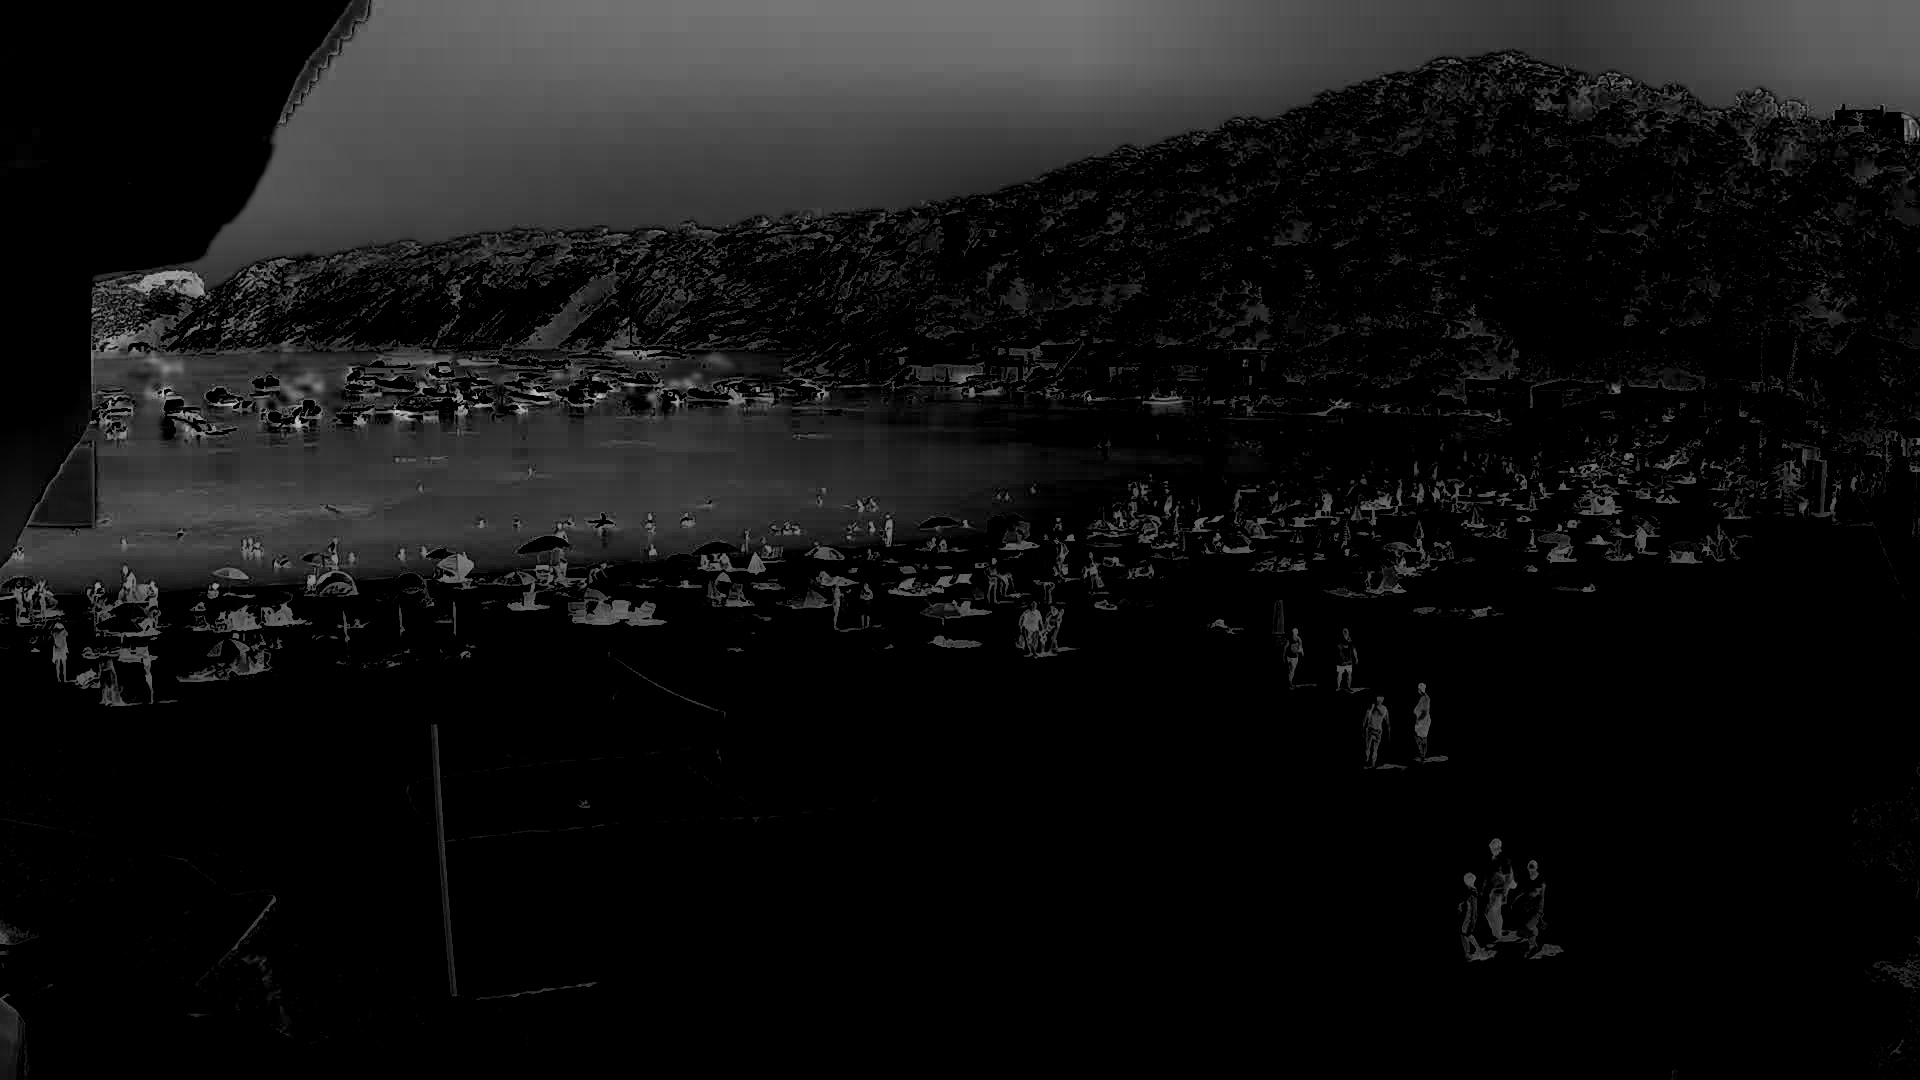
\includegraphics[width=\textwidth, height=\textheight, keepaspectratio]{img/sub.jpg}
    \caption{Image obtained by applying cv2.subtract(background, image)}
    \label{fig:sub}
  \end{figure}

  \begin{figure} [h]
    \centering
    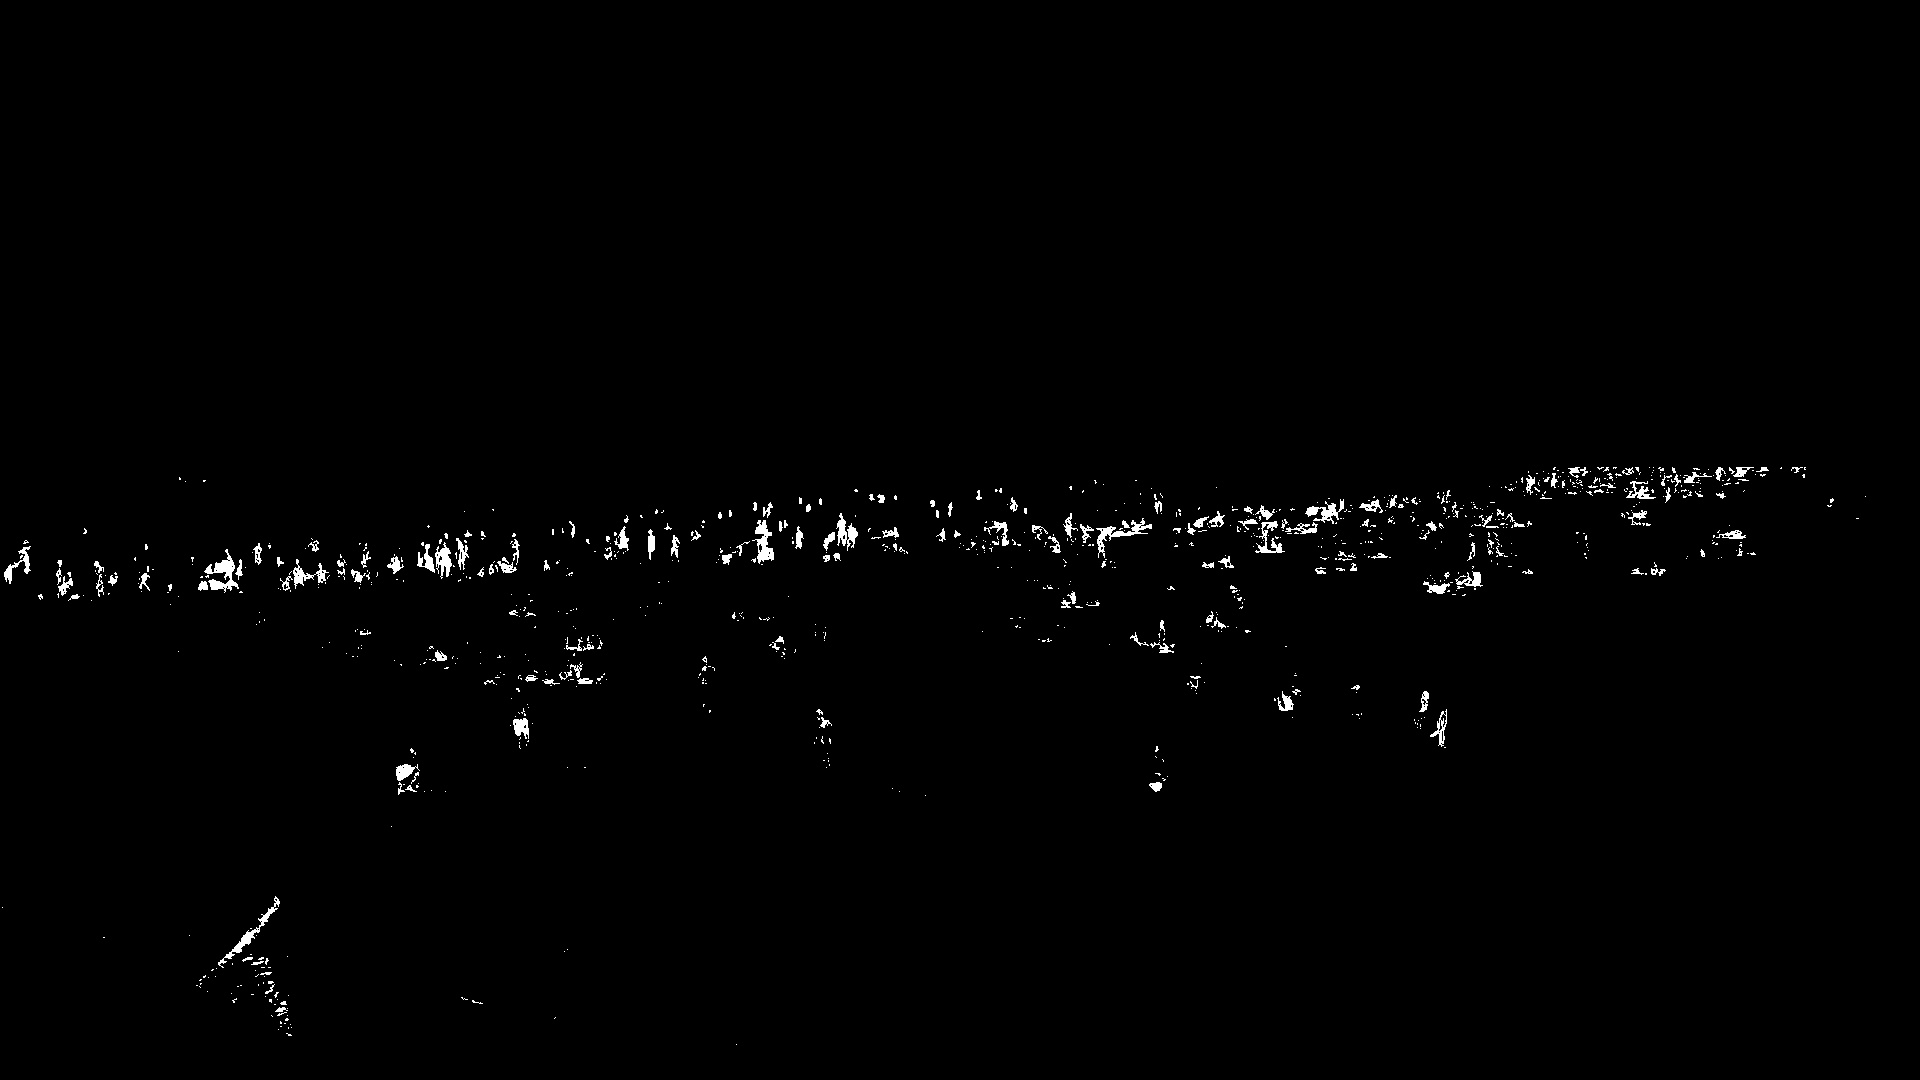
\includegraphics[width=\textwidth]{img/bin_th.jpg}
    \caption{Binarized image using a fix thresholding method}
    \label{fig:binth}
  \end{figure}

  \begin{figure} [h]
    \centering
    
\includegraphics[width=\textwidth]{../mask.png}
    \caption{Mask image}
    \label{fig:mask_ex}
  \end{figure}

  \begin{figure} [h]
    \centering
    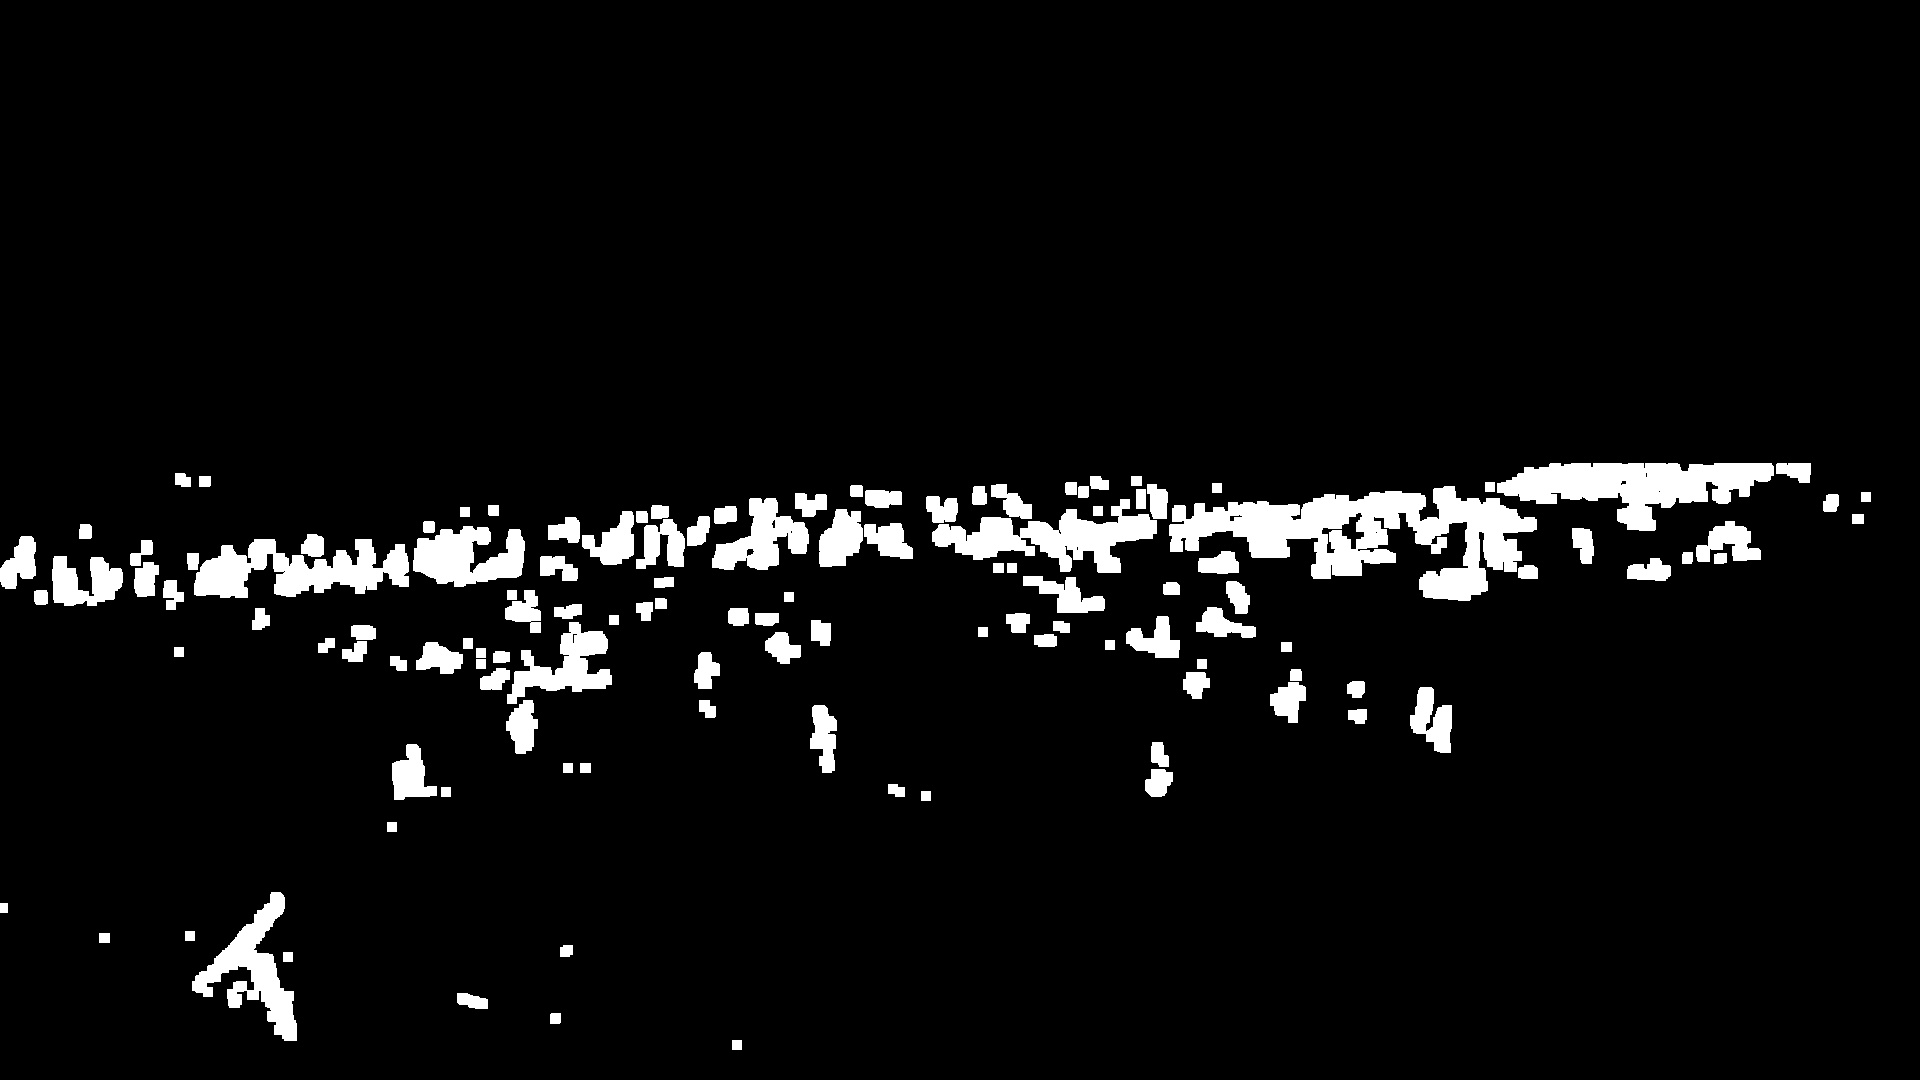
\includegraphics[width=\textwidth]{img/dil.jpg}
    \caption{Dilation applyed to the binarized image}
    \label{fig:dilation_ex}
  \end{figure}



  \section{Complementary Images}

  \begin{figure}[h]
    \centering
    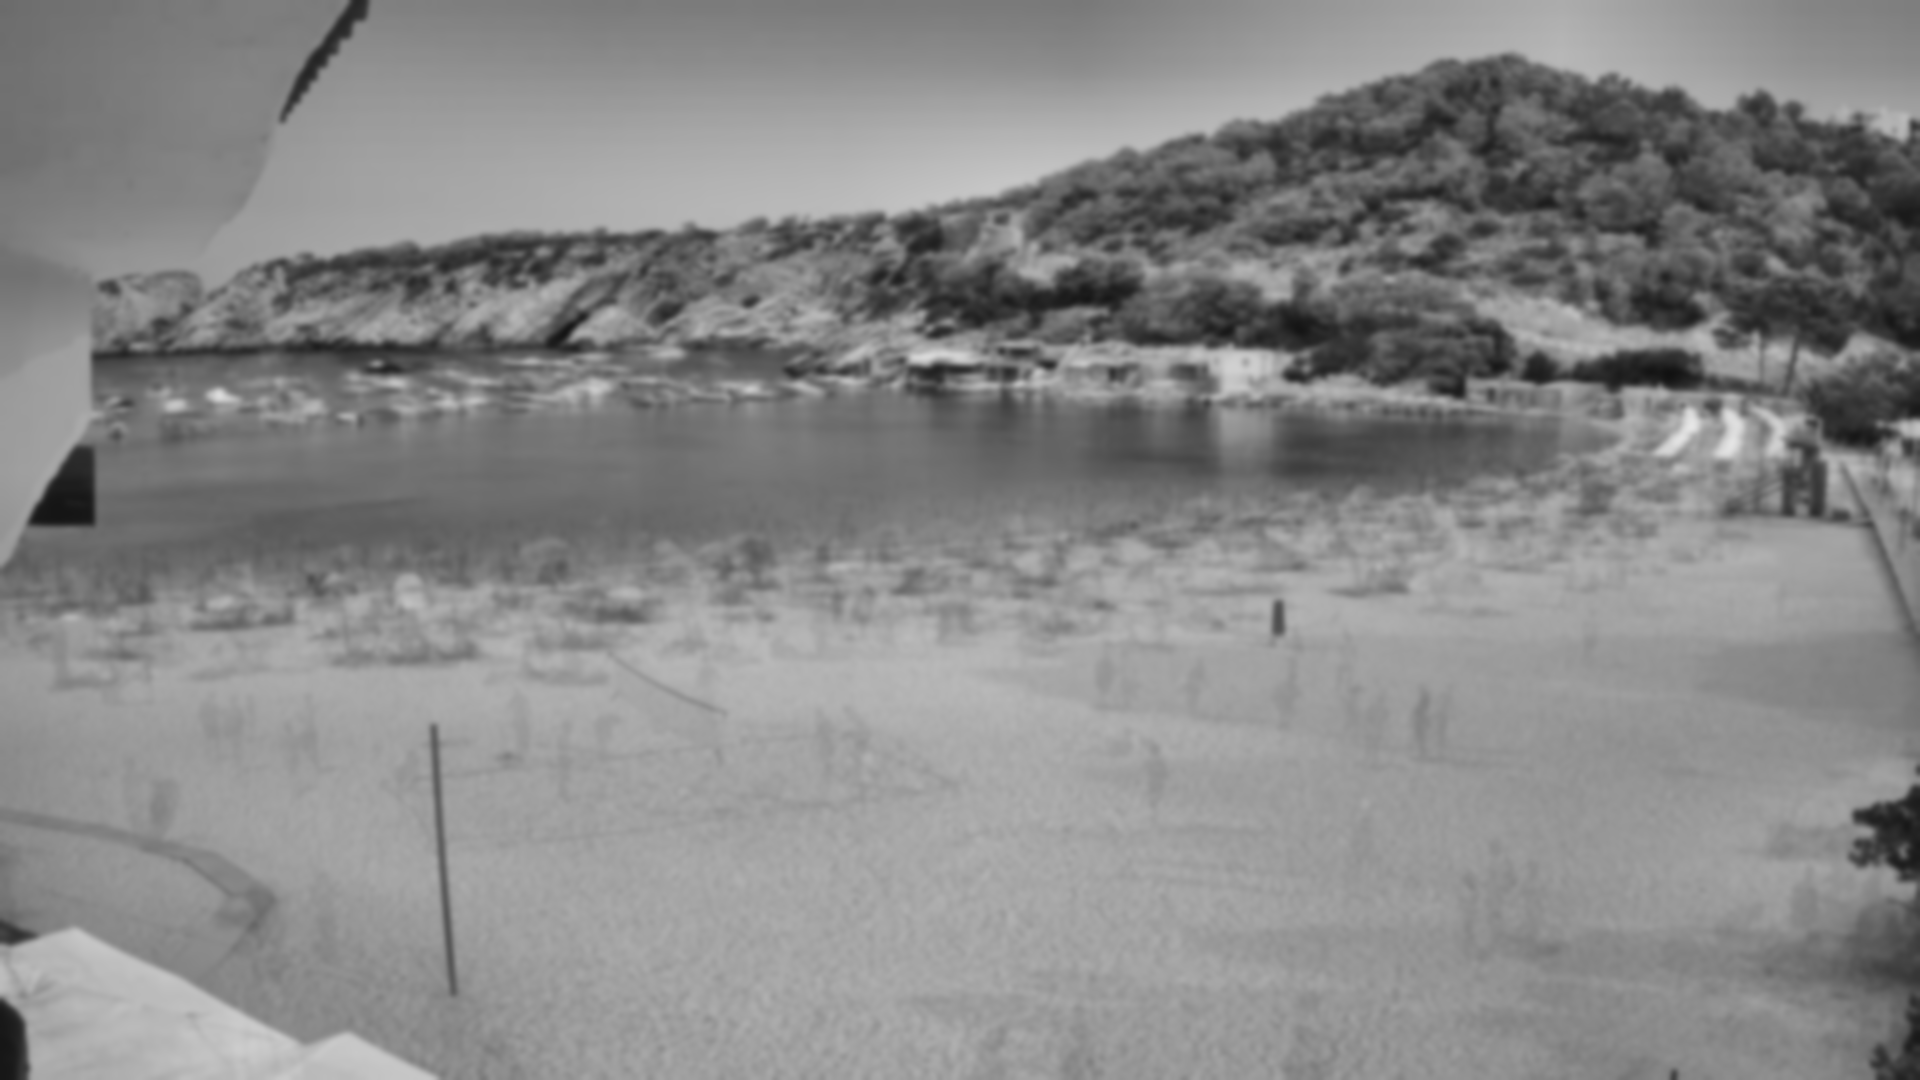
\includegraphics[width=0.9\textwidth]{img/avg.png}
    \caption{Average image with a gaussian blur applyed with a kernel of (11,11)}
    \label{fig:avg}
  \end{figure}

  \begin{figure}[h]
    \centering
    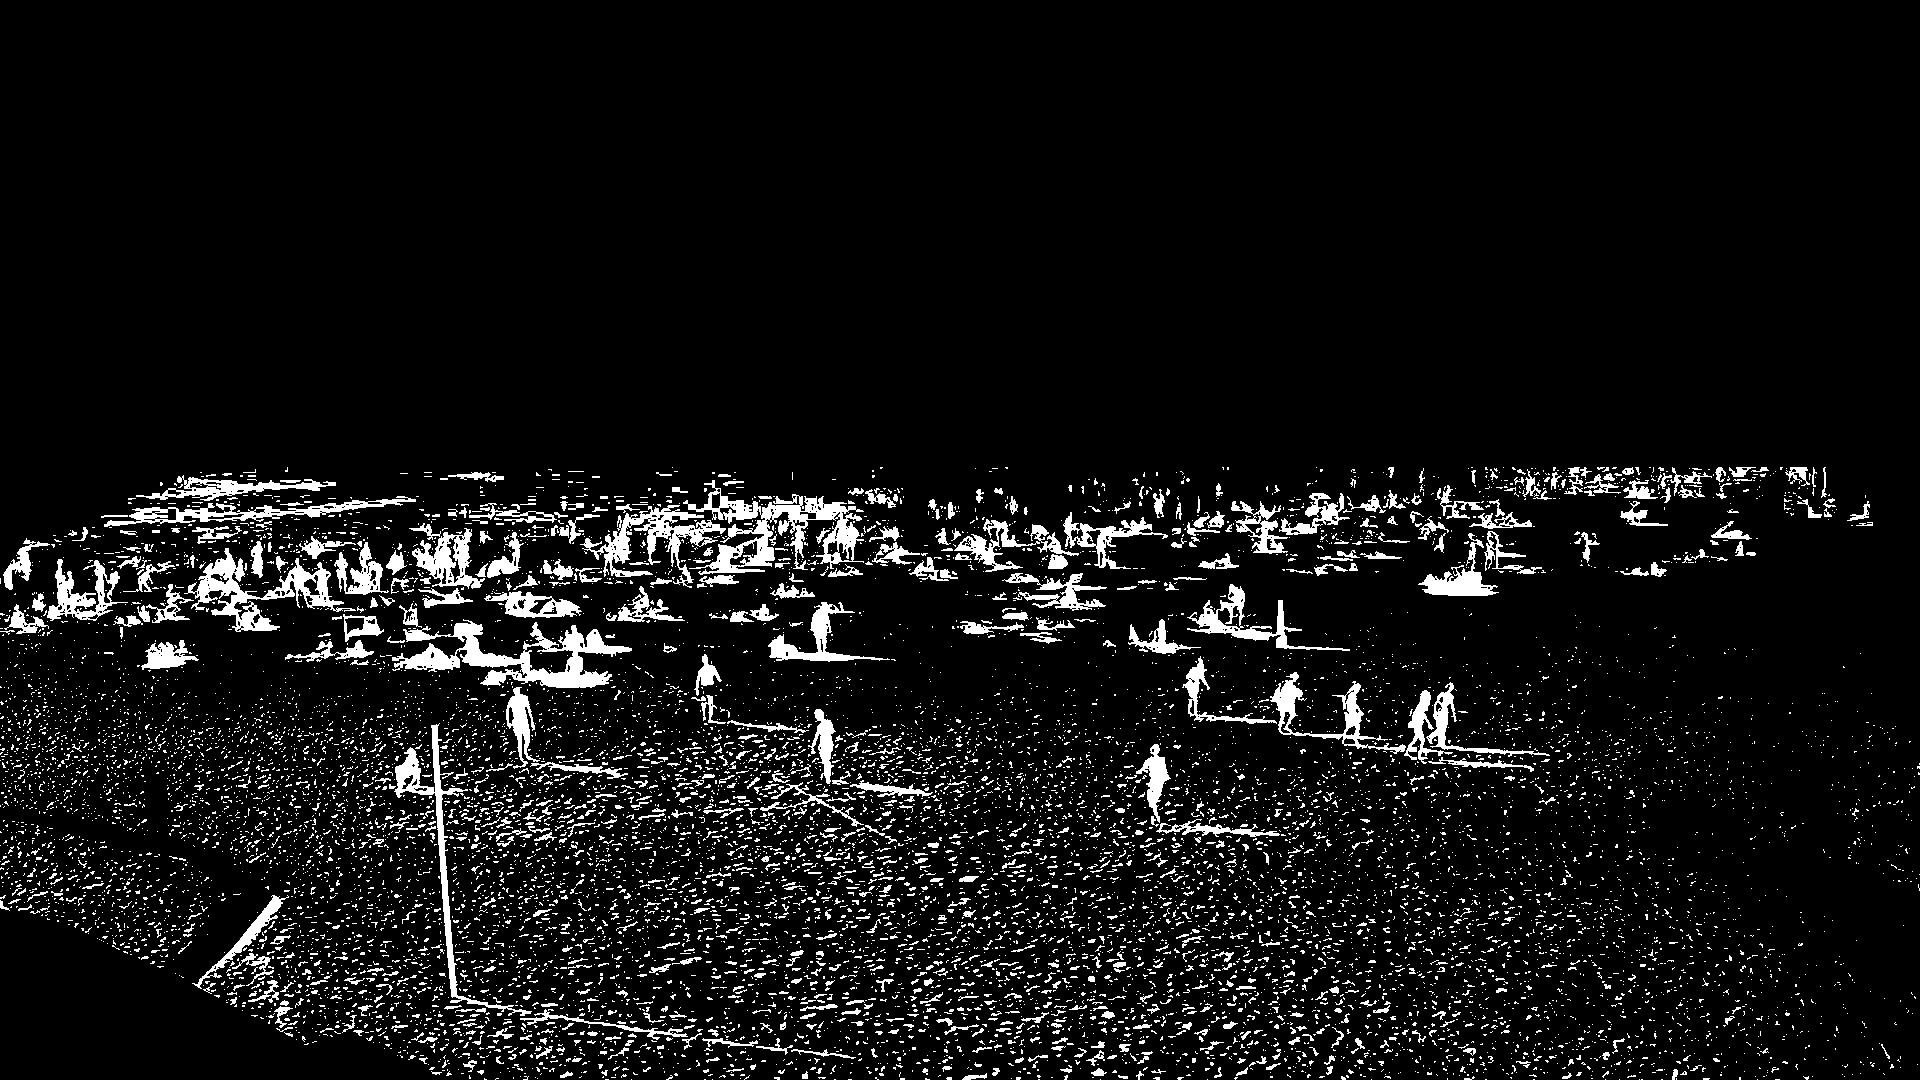
\includegraphics[width=\textwidth]{img/OTSU_sub_arena.jpg}
    \caption{Binarized image using OTSU and the empty beach image}
    \label{fig:otsu_bin}
  \end{figure}

\end{appendices}



\end{document}
